%%%%%%%%%%%%%%%%%%%%%%%%%%%%%%%%%%%%%%%%%
% TMDEI Dissertation
% LaTeX Template
% Version 0.1 (Dec/2015)
%
% Adapted to TMDEI/ISEP style (Dec/2015) by
%  Nuno Pereira (nap@isep.ipp.pt) and
%  Paulo Baltarejo (pbs@isep.ipp.pt)
%
% Based on MastersDoctoralThesis Version 1.2 by Vel (vel@latextemplates.com) and
% Johannes Böttcher, downloaded from (21/11/15):
% http://www.LaTeXTemplates.com
%
% This template is originally based on a template by:
% Steve Gunn (http://users.ecs.soton.ac.uk/srg/softwaretools/document/templates/)
% Sunil Patel (http://www.sunilpatel.co.uk/thesis-template/)
%
% Template license:
% CC BY-NC-SA 3.0 (http://creativecommons.org/licenses/by-nc-sa/3.0/)
%
%%%%%%%%%%%%%%%%%%%%%%%%%%%%%%%%%%%%%%%%%
%https://www.overleaf.com/project/5bfd7e508cfbf932785021c9
%----------------------------------------------------------------------------------------
%	PACKAGES AND OTHER DOCUMENT CONFIGURATIONS
%----------------------------------------------------------------------------------------

\documentclass[
11pt, % The default document font size, options: 10pt, 11pt, 12pt
%oneside, % Two side (alternating margins) for binding by default, uncomment to switch to one side (for drafting/reading purposes)
portuguese, % english for English;
%portuguese,% for Portuguese; delete temporary files if you change language (e.g. 'make clean; make')
singlespacing, % Single line spacing, alternatives: onehalfspacing or doublespacing (for drafting/reading purposes)
%draft, % Uncomment to enable draft mode (no pictures, no links, overfull hboxes indicated)
%nolistspacing, % If the document is onehalfspacing or doublespacing, uncomment this to set spacing in lists to single
liststotoc, % Uncomment to add the list of figures/tables/etc to the table of contents (recommended)
%toctotoc, % Uncomment to add the main table of contents to the table of contents (not recommended)
parskip, % Add space between paragraphs (recommended)
%nohyperref, % Uncomment to not load the hyperref package (not recommended)
nohyperreflinkcolor, % hyperref links are not colored (comment to color links, for example to produce an electronic-only version)
headsepline, % Uncomment to get a line under the header
]{tmdei-style} % The class file specifying the document structure

\usepackage{tikz} % Required for creating graphics programmatically (can be removed if not used)
%\usetikzlibrary{arrows} % Required for fancy arrows in TiKZ graphics (can be removed if not used)

\usepackage{pgfplots} % Required for drawing high--quality function plots (can be removed if not used)
\pgfplotsset{compat=newest}

%
% Next you have examples of admissable citation styles; we recomend using the authoryear-comp citation style (which resembles Harvard); don't forget to only uncomment one
%

% authoryear-comp: recommended citation style (e.g. (Buendía, 1860), (Buendía 1910, Arcadio 1940))
\usepackage[style=authoryear-comp,backend=biber]{biblatex} % Bibtex backend with the authoryear-comp citation style (authoryear citations, bibliography ordered alphabetically)

% numeric citation style (e.g. [1], [1-3])
%\usepackage[style=numeric-comp,sorting=none,backend=biber]{biblatex} % Bibtex backend with the numeric-comp citation style (numeric citations, bibliography ordered by appearance)

% alphabetic citation style (e.g. [Buendía10], [Buendía10, Arcadio40])
%\usepackage[style=alphabetic,sorting=none,backend=biber]{biblatex} % Bibtex backend with the alphabetic citation style (alphabetic citations, bibliography ordered by appearance)


\addbibresource{mainbibliography.bib} % The filename of the bibliography

\makeglossaries % build the glossary

%----------------------------------------------------------------------------------------
%	THESIS INFORMATION
%----------------------------------------------------------------------------------------

\thesistitle{SWBraille: Um simulador web da Máquina Braille} % Your thesis title, this is used in the title, print it elsewhere with \ttitle

%\thesissubtitle{{[}Thesis Subtitle{]}} % Your thesis title, this is used in the title, print it elsewhere with \tsubtitle

\author{David \textsc{Gomes de Jesus}} % Your name, this is used in the title page, print it elsewhere with \authorname

\subjectarea{Engenharia de Software} % Specialisation area (Computer Systems, Information and Knowledge Systems, Graphics, Systems and Multimedia, Software Engineering), used in the title page, print it elsewhere with \areaname

%\supervisor{Dra. Evaldinolia \textsc{Gilbertoni Moreira}}
\supervisor{Dra. Paula \textsc{Maria de Sá Oliveira Escudeiro}} % Your supervisor's name, this is used in the title page, print it elsewhere with \supname1

\cosupervisor{Dra. Evaldinolia \textsc{Gilbertoni Moreira}} % Your co-supervisor's name, this is used in the title page, print it elsewhere with \cosupname (comment, if no co-supervisor)

\committeepresident{Dra. Isabel Praça, Professora, DEI/ISEP} % Name of the president of the evaluation committee, print it elsewhere with \presidentname

%\committeemembers{
%    Dr. Jaimie Smith, Professor, DEI/ISEP\\
%    Dr. Jones Smith, Professor, DEI/ISEP\\
%    Dr. Jagger Smith, Professor, DEI/ISEP
%} % Name of the evaluation committee members (up to four), print it elsewhere with \committee

\keywords{braille, máquina, simulador, ensino, typewriter, simulator} % Please define up to 6 keywords that better describe your work, print it elsewhere with \keywordnames

\university{\href{https://www.isep.ipp.pt/}{Instituto Superior de Engenharia do Porto}} % Your university's name and URL, this is used in the title page and abstract, print it elsewhere with \univname

\department{\href{https://www.dei.isep.ipp.pt/}{Departamento de Engenharia Informática}} % Your department's name and URL, this is used in the title page and abstract, print it elsewhere with \deptname

\thesisdate{Porto, \today} % thesis date,  print it elsewhere with \tdate

\hypersetup{pdftitle=\ttitle} % Set the PDF's title to your title
\hypersetup{pdfauthor=\authorname} % Set the PDF's author to your name
\hypersetup{pdfkeywords=\keywordnames} % Set the PDF's keywords to your keywords

\begin{document}

%----------------------------------------------------------------------------------------
%	FRONT MATTER
%----------------------------------------------------------------------------------------

% Include the frontmatter of your thesis here
% we include the glossary here (frontmatter is included with \input, so this command is as if it was in main.tex)
%All acronyms must be written in this file.
\newacronym{RTS}{RTS}{Real-Time System}
\newacronym{GPOS}{GPOS}{General Purpose Operating System}
\newacronym{RTOS}{RTOS}{Real-Time Operating System}
\newacronym{PGF}{PGF}{Portable Graphics Format}


\frontmatter % Use roman page numbering style (i, ii, iii, iv...) for the pre-content pages

\pagestyle{plain} % Default to the plain heading style until the thesis style is called for the body content

%----------------------------------------------------------------------------------------
%	TITLE PAGE
%----------------------------------------------------------------------------------------

\maketitlepage


%----------------------------------------------------------------------------------------
%	STATEMENT of INTEGRITY
%----------------------------------------------------------------------------------------
\integritystatement

%----------------------------------------------------------------------------------------
%	DEDICATION  (optional)
%----------------------------------------------------------------------------------------
%
%\dedicatory{For/Dedicated to/To my\ldots}

%\begin{dedicatory}
%The dedicatory is optional. Below is an example of a humorous dedication.

%"To my wife Marganit and my children Ella Rose and Daniel Adam without whom this book would have been completed two years earlier." in "An Introduction To Algebraic Topology" by Joseph J. Rotman.
%\end{dedicatory}

%----------------------------------------------------------------------------------------
%	ABSTRACT PAGE
%----------------------------------------------------------------------------------------

\begin{abstract}

% here you put the abstract in the main language of the work.

O acesso à Máquina de escrever em Braille e o seu aprendizado tem sido desafiador dado aos altos valores das máquinas disponíveis à venda. Este trabalho apresenta o desenvolvimento de uma aplicação web que simula a Máquina Braille, a fim de proporcionar uma solução acessível para a prática e o aprendizado de Braille e da Máquina Braille. Para isso, a aplicação simula as teclas da máquina no teclado do computador, para que o usuário possa ter uma experiência que facilite a transição para o uso real da Máquina Braille.

A aplicação tem dois modos: o Modo Livre, onde permite aos usuários usarem livremente o simulador e visualizar os textos escritos em células Braille, e o Modo de Lições, onde é oferecido vários exercícios e lições visando facilitar o aprendizado do Sistema Braille e da Máquina Braille. Além disso, a ferramenta inclui a funcionalidade de visualizar o texto a tinta, facilitando usuários menos familiarizados com o Braille.

Este estudo contribui para a acessibilidade e inclusão de pessoas com deficiência visual, principalmente aquelas que adquiriram a deficiência recentemente, pois oferece uma solução prática e eficaz para o aprendizado do Braille. Permitir que os usuários pratiquem a Máquina Braille de forma virtual e interativa é facilitar a transição para o uso real da Máquina Braille, assim, promovendo autonomia e independência das pessoas com deficiência visual.

\end{abstract}

\begin{abstractotherlanguage}
% here you put the abstract in the "other language": English, if the work is written in Portuguese; Portuguese, if the work is written in English.

Access to the Braille typewriter and learning it has been challenging due to the high prices of the machines available for sale. This work presents the development of a web application that simulates the Braille Machine, aiming to provide an affordable solution for practicing and learning Braille and the Braille Machine. The application simulates the machine's keys on the computer keyboard, allowing the user to have an experience that facilitates the transition to using the Braille Machine in real life.

The application has two modes: Free Mode, which allows users to freely use the simulator and view the texts written in Braille cells, and Lesson Mode, which offers various exercises and lessons to facilitate learning of the Braille System and the Braille Machine. Additionally, the tool includes the functionality to view the text in ink, making it easier for users less familiar with Braille.

This study contributes to the accessibility and inclusion of people with visual impairments, especially those who have recently acquired the impairment, as it offers a practical and effective solution for learning Braille. Allowing users to practice the Braille Machine virtually and interactively facilitates the transition to using the Braille Machine in real life, thus promoting autonomy and independence for people with visual impairments.


\end{abstractotherlanguage}

%----------------------------------------------------------------------------------------
%	ACKNOWLEDGEMENTS (optional)
%----------------------------------------------------------------------------------------

%\begin{acknowledgements}

%The optional Acknowledgment goes here\ldots Below is an example of a humorous acknowledgment.

%"I'd also like to thank the Van Allen belts for protecting us from the harmful solar wind, and the earth for being just the right distance from the sun for being conducive to life, and for the ability for water atoms to clump so efficiently, for pretty much the same reason. Finally, I'd like to thank every single one of my forebears for surviving long enough in this hostile world to procreate. Without any one of you, this book would not have been possible." in "The Woman Who Died a Lot" by Jasper Fforde.
%\end{acknowledgements}

%----------------------------------------------------------------------------------------
%	LIST OF CONTENTS/FIGURES/TABLES PAGES
%----------------------------------------------------------------------------------------

\tableofcontents % Prints the main table of contents

\listoffigures % Prints the list of figures

\listoftables % Prints the list of tables

\iflanguage{portuguese}{
\renewcommand{\listalgorithmname}{Lista de Algor\'itmos}
}
\listofalgorithms % Prints the list of algorithms
\addchaptertocentry{\listalgorithmname}


\renewcommand{\lstlistlistingname}{List of Source Code}
\iflanguage{portuguese}{
\renewcommand{\lstlistlistingname}{Lista de C\'odigo}
}
\lstlistoflistings % Prints the list of listings (programming language source code)
\addchaptertocentry{\lstlistlistingname}


%----------------------------------------------------------------------------------------
%	ABBREVIATIONS
%----------------------------------------------------------------------------------------
%\begin{abbreviations}{ll} % Include a list of abbreviations (a table of two columns)
%%\textbf{LAH} & \textbf{L}ist \textbf{A}bbreviations \textbf{H}ere\\
%%\textbf{WSF} & \textbf{W}hat (it) \textbf{S}tands \textbf{F}or\\
%\end{abbreviations}

%----------------------------------------------------------------------------------------
%	SYMBOLS
%----------------------------------------------------------------------------------------

\begin{symbols}{lll} % Include a list of Symbols (a three column table)

%$a$ & distance & \si{\meter} \\
%$P$ & power & \si{\watt} (\si{\joule\per\second}) \\
%Symbol & Name & Unit \\

%\addlinespace % Gap to separate the Roman symbols from the Greek

%$\omega$ & angular frequency & \si{\radian} \\

\end{symbols}



%----------------------------------------------------------------------------------------
%	ACRONYMS
%----------------------------------------------------------------------------------------

\newcommand{\listacronymname}{List of Acronyms}
\iflanguage{portuguese}{
\renewcommand{\listacronymname}{Lista de Acr\'onimos}
}

%Use GLS
\glsresetall
\printglossary[title=\listacronymname,type=\acronymtype,style=long]

%----------------------------------------------------------------------------------------
%	DONE
%----------------------------------------------------------------------------------------

\mainmatter % Begin numeric (1,2,3...) page numbering
\pagestyle{thesis} % Return the page headers back to the "thesis" style


%----------------------------------------------------------------------------------------
%	MAIN BODY
%----------------------------------------------------------------------------------------

% Include the chapters of the thesis as separate folder for each chapter
% Uncomment the lines as you write the chapters


% % Chapter 1
% 
\chapter{Introdução} % Main chapter title
\label{chap:Chapter01} % For referencing the chapter elsewhere, use Chapter~\ref{Chapter01}
%-------------------------------------------------------------------------------
%---------
%

\section{Contexto} 
\label{sec:chap01_context} %For referencing this section elsewhere, use Section~\ref{sec:chap1_introduction}

A alfabetização em Braille é um fator de extrema importância para a independência e inclusão de pessoas com deficiência visual \parencite{REF01}. O sistema Braille, inventado por Louis Braille no século XIX \parencite{REF02}, é amplamente utilizado em todo o mundo como método de leitura e escrita para cegos, permitindo que essas pessoas acessem informação e comunicação de forma eficaz.

Nos últimos anos, tem havido um crescente reconhecimento da importância da acessibilidade e inclusão para pessoas com deficiência visual. O aprendizado do Braille e o acesso a ferramentas como a máquina de escrever em Braille desempenham um papel fundamental na promoção da independência e autonomia dessas pessoas, não apenas na educação, mas também no trabalho e na vida cotidiana. No entanto, a aprendizagem do Braille não é isenta de desafios. O elevado custo das máquinas Braille e a escassez de unidades disponíveis em muitos contextos educacionais ou de reabilitação dificultam o acesso e a prática, criando barreiras para o aprendizado \parencite{REF01}.

Em ambientes educacionais e de reabilitação, onde o ensino do Braille é fundamental, a necessidade de múltiplas máquinas de escrever para atender a vários alunos representa uma barreira significativa, tanto em termos de recursos financeiros quanto de infraestrutura. A limitação no número de máquinas Braille em instituições de ensino ou reabilitação pode restringir a prática individual dos alunos, prejudicando o ritmo de aprendizado e a autonomia dos estudantes.

Nesse cenário, surge a necessidade do desenvolvimento de ferramentas acessíveis e inovadoras que permitam a prática do Braille de forma mais econômica e eficiente e que facilitem o acesso às máquinas de escrever em Braille. É nesse contexto que se insere este trabalho, que propõe o desenvolvimento de uma aplicação web e gratuita, que simula o funcionamento da máquina de escrever em Braille.

A aplicação proposta visa superar algumas das limitações das máquinas de escrever em Braille tradicionais, oferecendo uma alternativa acessível, prática e eficaz para o aprendizado e prática do Braille. Simulando as funcionalidades de uma máquina de escrever em Braille através do teclado do computador, a aplicação permite que os usuários pratiquem o Braille de forma virtual e interativa, facilitando a transição para o uso real da máquina Braille.

Além disso, a aplicação oferece a visualização do texto em tinta, tornando o conteúdo acessível para usuários que não estão familiarizados com o Braille. Com isso, o trabalho proposto contribui não apenas para a melhoria da acessibilidade e inclusão de pessoas com deficiência visual, mas também para a promoção do aprendizado e uso do Braille em um contexto mais amplo.

\section{Problema}

O aprendizado do Braille e o acesso às máquinas de escrever em Braille representam desafios significativos para pessoas com deficiência visual, especialmente para aqueles que ficaram cegos recentemente. A escassez de recursos acessíveis e o valor elevado das Máquinas Braille dificultam o acesso a ferramentas adequadas para o aprendizado e prática do Braille \parencite{REF01}. Além disso, a necessidade de múltiplas máquinas de escrever em Braille para práticas em grupo, como em ambientes educacionais, representa uma barreira adicional para o acesso e a inclusão de pessoas com deficiência visual.

Assim, surge a necessidade de desenvolver soluções inovadoras e acessíveis que facilitem o aprendizado do Braille e o acesso às máquinas de escrever em Braille de forma mais eficaz e inclusiva. A necessidade de uma solução que permita a prática virtual, de baixo custo e acessível, é o ponto central abordado por esta dissertação, que visa contribuir com a criação de um ambiente inclusivo para o aprendizado e a prática do Braille, facilitando o acesso de pessoas com deficiência visual a essas ferramentas fundamentais.

Diante desse problema, surge a seguinte questão: Como desenvolver uma aplicação web simuladora da máquina de escrever em Braille que seja acessível, prática e eficaz para o aprendizado e prática do Braille, contribuindo assim para a promoção da inclusão e autonomia de pessoas com deficiência visual?




\section{Objetivos}

\subsection{Objetivo Geral}

Desenvolver uma aplicação web gratuita que simule a máquina de escrever em Braille, oferecendo uma ferramenta acessível, prática e eficaz para o aprendizado e prática do sistema Braille. O projeto visa promover a inclusão e autonomia de pessoas com deficiência visual, facilitando o acesso ao ensino e à prática do Braille, especialmente para aqueles que enfrentam barreiras financeiras e tecnológicas ao utilizar máquinas Braille físicas.

\subsection{Objetivos específicos}

\begin{itemize}
    \item Projetar e implementar uma interface acessível e intuitiva, assegurando usabilidade para pessoas com deficiência visual, com uma experiência fluida e amigável para todos os usuários, seguindo boas práticas de acessibilidade web.

    \item Desenvolver algoritmos que simulem as funcionalidades da máquina de escrever em Braille, mapeando as teclas do teclado do computador para os pontos Braille correspondentes, permitindo uma experiência de digitação próxima com a real.

    \item Implementar o Modo Livre, que permite aos usuários praticarem a escrita em Braille de forma livre, com a visualização das células Braille correspondentes diretamente na tela.

    \item Desenvolver o Modo Desafio, no qual são apresentadas palavras para que o usuário pratique digitando-as corretamente, com feedback imediato, promovendo o aprendizado de forma interativa e envolvente.

    \item Integrar funcionalidades adicionais, como a visualização do texto em tinta, para facilitar o uso por pessoas que não são familiarizadas com o sistema Braille, ampliando o alcance e a acessibilidade da aplicação.

    \item Realizar testes e avaliações com usuários com deficiência visual, assegurando que a aplicação atenda aos critérios de eficácia, acessibilidade e usabilidade, permitindo ajustes e melhorias baseados em feedback real.

    \item Avaliar o impacto da aplicação no aprendizado e prática do Braille, medindo como ela contribui para a promoção da inclusão e autonomia de pessoas com deficiência visual, e identificando melhorias contínuas para maximizar esses benefícios.

\end{itemize}

Atingindo esses objetivos, espera-se que a aplicação desenvolvida neste trabalho se torne uma ferramenta valiosa para o aprendizado e prática do sistema Braille. Com isso, o projeto contribuirá para a inclusão social e para a promoção da autonomia de pessoas com deficiência visual, oferecendo uma solução acessível e eficaz.

\section{Questões de Investigação}

Para orientar o desenvolvimento deste trabalho e garantir que os objetivos propostos sejam alcançados, é necessário levantar questões-chave que guiarão o processo de pesquisa. Essas questões de investigação buscam explorar os desafios e oportunidades relacionados ao aprendizado e à prática do sistema Braille por meio de uma aplicação web que simule uma máquina de escrever em Braille. Elas também visam compreender como a o projeto pode contribuir para a inclusão e a autonomia de pessoas com deficiência visual.

\begin{table}[h]
    \caption{Questão global}
    \label{tab:ch01-global-question}
    \centering
    \begin{tabular}{c>{\raggedright\arraybackslash}p{0.8\linewidth}}
        \toprule
        \tabhead{Questão}& \tabhead{Questão de Investigação}\\
        \midrule
        Qg& Como a aplicação pode contribuir para democratizar o aprendizado do Braille e da máquina de escrever Braille, promovendo autonomia a pessoas com deficiência visual?\\
        \bottomrule\\
    \end{tabular}
\end{table}

A questão global, descrita na tabela \ref{tab:ch01-global-question}, norteia toda a pesquisa e busca compreender o impacto que a aplicação pode ter na democratização do uso da Máquina Braille e na melhoria do ensino de Braille a pessoas com ou sem deficiência visual. A investigação dessa questão permitirá avaliar como a ferramenta pode tornar o aprendizado do Braille mais acessível e eficiente, especialmente para aqueles que enfrentam barreiras financeiras e tecnológicas. A resposta a essa questão será determinante para avaliar a relevância e o impacto do estudo, confirmando sua contribuição para a inclusão social e a promoção da independência de seus usuários.

Além da questão global que orienta o desenvolvimento deste trabalho, foram definidas três questões específicas que visam detalhar aspectos fundamentais da pesquisa. Essas questões buscam avaliar a eficácia, as funcionalidades e o impacto da aplicação no aprendizado do Braille e na promoção da inclusão de pessoas com deficiência visual.

\begin{table}[h]
    \caption{Questões específicas}
    \label{tab:ch01-specific-questions}
    \centering
    \begin{tabular}{c>{\raggedright\arraybackslash}p{0.8\linewidth}}
        \toprule
        \tabhead{Questão}& \tabhead{Questão de Investigação}\\
        \midrule
        Qe1& Quais as características e funcionalidades que a tornam uma alternativa mais acessível e eficaz para o aprendizado da máquina Braille?\\
        \addlinespace
        Qe2& A aplicação é eficaz no ensino do Braille e da máquina de escrever Braille para usuários com diferentes níveis de conhecimento?\\
        \addlinespace
        Qe3& Qual é o impacto da aplicação no aprendizado e prática do Braille, bem como na promoção da inclusão e autonomia de pessoas com deficiência visual, e como esse impacto pode ser avaliado e quantificado?\\
        \bottomrule\\
    \end{tabular}
\end{table}

A Qe1 foca em identificar os elementos que fazem da aplicação uma solução viável em termos de acessibilidade e eficiência. Nessa questão, a investigação busca entender quais funcionalidades da simulação da máquina de escrever em Braille proporcionam uma experiência de aprendizado adequada, além de explorar os fatores que tornam essa solução mais econômica e prática em comparação com as máquinas Braille físicas. A resposta a esta questão irá fornecer informações sobre o potencial da aplicação para democratizar o acesso ao Braille. 

A Qe2 aborda a eficácia pedagógica da aplicação. Será analisado como a ferramenta atende tanto a iniciantes quanto a usuários mais avançados no aprendizado do Braille. A investigação nessa questão visa identificar se a aplicação pode ser usada como uma ferramenta inclusiva e flexível, capaz de adaptar-se a diferentes perfis de usuários e seus respectivos níveis de conhecimento. Ao investigar como a ferramenta pode se adaptar a diversos perfis de aprendizado, essa questão permitirá entender o alcance e a versatilidade da aplicação como um recurso educacional inclusivo.

Por fim, a Qe3 trata de medir o impacto real da aplicação no processo de aprendizado e inclusão. Serão analisados os benefícios gerados em termos de autonomia e qualidade de ensino para as pessoas com deficiência visual, bem como o efeito no aprendizado do Braille. A pesquisa também se concentrará em desenvolver formas de avaliação e quantificação desse impacto, considerando métricas como progresso no aprendizado, feedback de usuários e melhorias na capacidade de utilizar a máquina Braille real.

%\chapter{Estado da Arte} 
\label{chap:Chapter02} 

\section{Sistema Braille}

\subsection{História do Braille}

Braille é um sistema de escrita tátil que permite às pessoas com deficiência visual ler e escrever de forma independente. Desenvolvido pelo francês Louis Braille no século XIX \parencite{REF02}, o sistema utiliza uma série de pontos em relevo dispostos em células de seis pontos. Com isso, o Braille é capaz de representar letras, números, símbolos matemáticos e até mesmo partituras musicais. 

\begin{figure}[h]
    \centering
    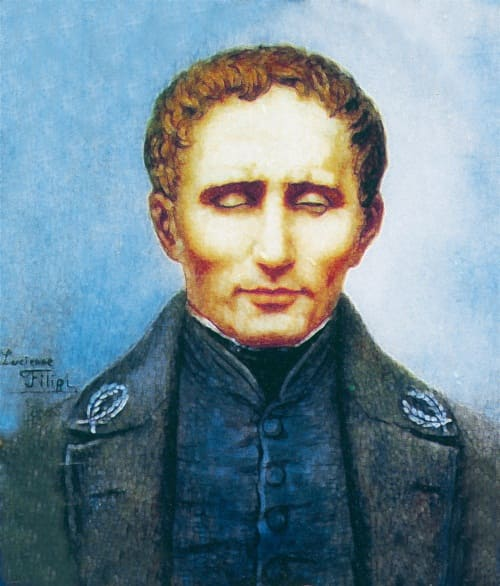
\includegraphics[scale=0.5]{ch02/assets/louis-braille.jpg}
    \decoRule
    \caption[Louis Braille]{Louis Braille, criador do Sistema Braille \parencite{IMG01}}
    \label{fig:ch02-braille-history-louis-braille}
\end{figure}

Na época, era utilizado o sistema Valentin Haüy \parencite{REF03}, que consistia em imprimir livros com a fonte bem ampliada e em relevo, possibilitando assim a leitura, mas não a escrita. Louis decidiu então buscar uma solução em um método que permitisse de forma prática e com poucas combinações a leitura e escrita para pessoas com deficiência visual.

Em 1824, Louis concluiu o desenvolvimento da base de seu sistema, aos 15 anos de idade. Ao longo dos anos continuou aprimorando, e em 1839 sua última publicação explicando o seu método foi muito bem recebida por parte dos alunos do Instituto Nacional para Jovens Cegos. Então, em 1843, o sistema Braille foi oficialmente adotado pelo instituto e passou a ser difundido por toda a Europa \parencite{REF03}.

Em 1852, Louis Braille faleceu aos 43 anos, devido a complicações de tuberculose. Louis deixou um legado duradouro \parencite{REF03}. Seu sistema de escrita tátil revolucionou a comunicação de pessoas com deficiência visual. Além de permitir o acesso à informação escrita, o sistema Braille até hoje promove igualdade de oportunidades educacionais e profissionais, permitindo seus usuários participarem ativamente da sociedade.

\subsection{Funcionamento do Sistema Braille}

O Braille é composto por unidades básicas denominadas de “celas” ou “células” que são compostas por uma matriz de pontos dispostos em duas colunas verticais. Cada célula pode conter de zero a seis pontos, numerados de 1 a 6. Os pontos são organizados em duas colunas, com três pontos em cada coluna. Assim, os pontos da esquerda de cima para baixo são os pontos 1, 2 e 3, e os da direita são os pontos 4, 5 e 6 \parencite{REF04}.

\begin{figure}[h]
    \centering
    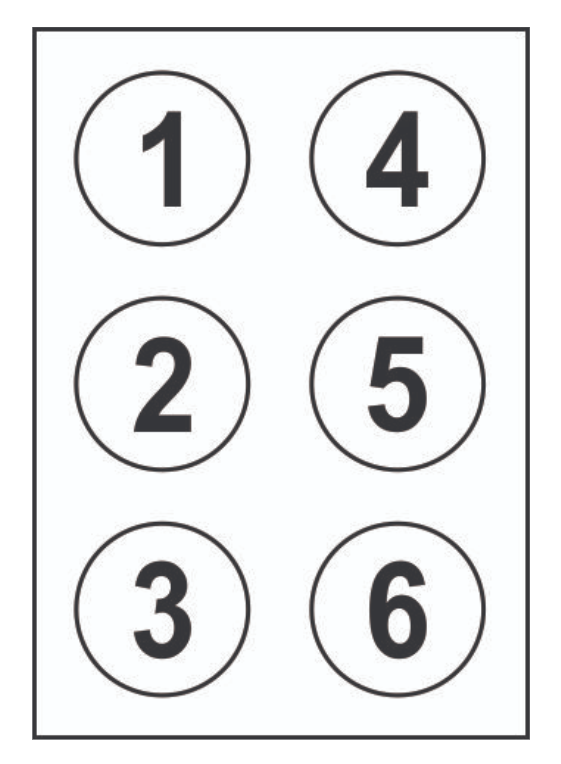
\includegraphics[scale=0.4]{ch02/assets/braille-cell.png}
    \decoRule
    \caption[Cela Braille]{Cela Braille}
    \label{fig:ch02-braille-cell}
\end{figure}

Cada combinação de pontos dentro da cela pode representar um caractere específico ou uma convenção adotada no Braille. Existem um total de 64 combinações possíveis, incluindo a cela totalmente vazia. Celas individuais ou a combinação de celas permitem o Braille representar letras do alfabeto, números, símbolos matemáticos, sinais de pontuação, palavras, frases e até mesmo textos inteiros \parencite{REF05}.

\begin{figure}[h]
    \centering
    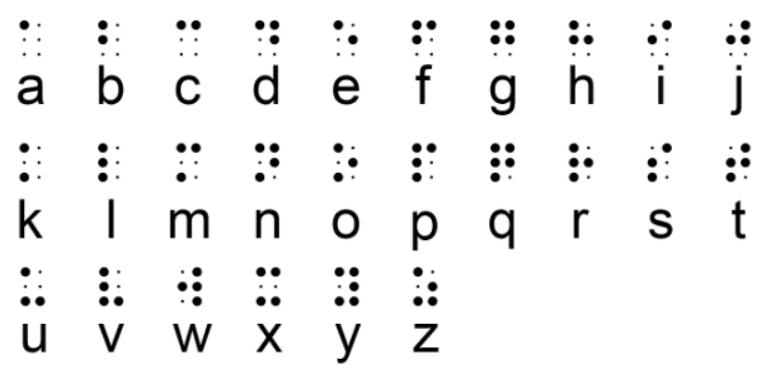
\includegraphics[scale=0.5]{ch02/assets/braille-alphabet.png}
    \decoRule
    \caption[Alfabeto em Braille]{Alfabeto em Braille}
    \label{fig:ch02-braille-alphabet}
\end{figure}

Para ler um texto Braille, uma pessoa utiliza as pontas dos dedos para sentir os pontos em relevo em alguma superfície. Cada cela é sentida e lida individualmente e, com prática, os leitores de Braille são capazes de fazer a leitura rapidamente. Já para a escrita em Braille, há diversas técnicas. O uso de uma reglete e um punção é uma das formas mais comuns de se escrever em Braille, onde o usuário pressiona pontos em uma folha de papel especial para criar pontos em relevo.

A máquina de escrever em Braille também é uma das formas mais comuns e tradicionais de gerar textos em Braille. Ela é especialmente projetada para permitir que pessoas cegas ou com baixa visão escrevam em Braille de forma eficiente e precisa. Seu funcionamento se assemelha a máquina de escrever convencional, porém com menos teclas e produzindo pontos em relevo para formar as celas Braille.

\section{Máquina Braille}

\subsection{Visão Geral}

Em 1892, o americano Frank Haven Hall pensou na primeira máquina própria para escrever em Braille. Em 1951, surgiu a Máquina Perkins, desenvolvida por um carpinteiro que trabalhava na Perkins School for the Blind, David Abraham. A máquina tem um funcionamento bem simples e intuitivo, além de muito parecido com uma máquina de escrever tradicional

\begin{figure}[h]
    \centering
    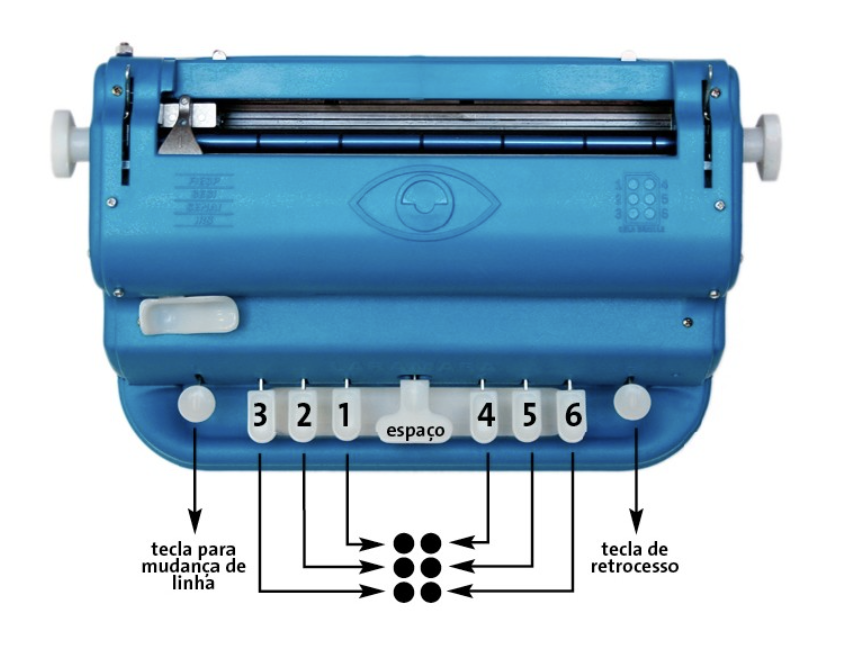
\includegraphics[scale=0.5]{ch02/assets/braille-typewriter.png}
    \decoRule
    \caption[Máquina Braille]{Máquina Braille com as teclas sinalizadas}
    \label{fig:ch02-braille-typewriter}
\end{figure}

Consistem em sete teclas principais, sendo que seis delas representam cada ponto de uma cela Braille e uma que representa uma cela vazia. Quando uma tecla é pressionada, o ponto correspondente é perfurado em um papel colocado atrás da máquina, criando assim o texto em Braille. Algumas máquinas também incluem características adicionais, como ajuste de espaçamento entre as células e a capacidade de produzir caracteres em negrito para ênfase.

Essas máquinas são muito importantes para pessoas com deficiência visual, seu uso se torna crucial no meio acadêmico e profissional, pois lhes permite criar documentos e ter acesso a informações de forma independente. As máquinas Braille vêm tendo avanços tecnológicos, com máquinas cada vez mais sofisticadas e integradas a outros dispositivos eletrônicos.

\subsection{Valores da Máquina Braille}
\label{sec:ch02_Valores_da_Maquina_Braille}

Apesar da importância da máquina Braille para as pessoas com deficiência visual, um dos principais obstáculos para a aquisição desse equipamento é o seu custo elevado. Uma busca no site oficial da Perkins, uma das mais renomadas fabricantes desse dispositivo, mostra que as máquinas de escrever em Braille estão longe de serem acessíveis para a maioria das pessoas, pois os preços são bem expressivos. Por exemplo, uma Máquina Braille comum é vendida por \$810, enquanto uma Máquina Braille Inteligente chega a \$2.195,00. Convertendo esses valores para real e euro, temos que a Máquina Braille Comum custa R\$3.996,54 ou 746,78€. Já a Máquina Braille Inteligente custa R\$10.829,91 ou 2.023,61€.

Diante disso, torna-se compreensível que a maioria indivíduos com deficiência visual tenham dificuldade ao tentar adquirir uma Máquina Braille. O alto custo desse equipamento torna a compra praticamente inviável para muitas pessoas, especialmente aquelas com recursos financeiros mais limitados. Instituições de ensino de Braille também se tornam afetadas nesse cenário, já que não é muito viável a compra de vários exemplares para disponibilizar para os alunos. Assim, a alternativa de investir em outras tecnologias, como computadores ou notebooks, parece ser mais atrativa.

\section{Trabalhos relacionados}

\subsection{BrailleType}

No BrailleType \parencite{REF06}, a interface consiste em 6 botões ordenados em 2 colunas. Esse botões são colocados nas bordas e cantos da tela para facilitar sua localização. Os pontos são escolhidos um por um em qualquer ordem com confirmação de áudio. O BrailleType permite que o usuário cego insira texto como se estivesse escrevendo Braille usando o tradicional código matricial de 6 pontos.

\begin{figure}[h]
    \centering
    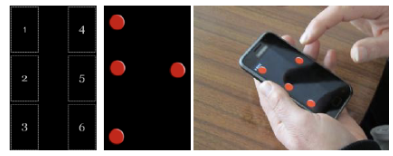
\includegraphics{ch02/assets/brailletype.png}
    \decoRule
    \caption[Interface do BrailleType]{Tela principal do BrailleType à esquerda. Ao centro mostra a letra 'r' marcada e pronta para ser confirmada. À direita um usuário escrevendo a letra 'r' no BrailleType. \parencite{REF06}}
    \label{fig:ch02-brailletype}
\end{figure}

Todas as interações com BrailleType são feitas usando apenas um único dedo. Sempre que um usuário pressiona ou arrasta um dedo para um novo ponto, o número do ponto correspondente é anunciado de forma audível, mas o ponto não é selecionado imediatamente. Há um pequeno tempo a se esperar para evitar seleções involuntárias do usuário. Este tempo pode ser facilmente configurado, permitindo que um usuário mais experiente diminua ou elimine a espera. 

Então, para marcar um ponto na célula Braille, o usuário deve tocar no alvo desejado e aguardar um sinal sonoro de confirmação. Repetindo o processo em um ponto já marcado o remove e informa ao usuário por meio de feedback de áudio. Após marcar todos os pontos necessários para um caractere Braille, na ordem que o usuário desejar, um duplo toque em qualquer parte da tela confirma a inserção. Se o usuário tentar aceitar uma combinação incorreta de pontos, a matriz Braille será apagada e um som de erro será reproduzido.

Esta aplicação oferece uma abordagem menos estressante com dispositivos com tela sensível ao toque, reduzindo o número de toques na tela. Ao reduzir o número de erros e permitir que o usuário tenha sucesso, sua confiança aumenta. Além de aproveitar as capacidades daqueles que usam Braille regularmente, também permite que aqueles que não o fazem aprendam ou mantenham o uso do Braille através de interações diárias simples.

\subsection{SingleTapBraille}

O principal objetivo do SingleTapBraille \parencite{REF07} foi desenvolver um novo método de entrada de texto que elimine a necessidade de os usuários encontrarem locais específicos para inserir letras, permitindo que as informações sejam inseridas de maneira rápida e eficaz usando um único polegar ou dedo. O objetivo buscou identificar as melhores funcionalidades para usuários que estão restritos a usar apenas uma mão para realizar tarefas em seu dispositivo móvel. Uma conclusão preliminar do estudo foi que a maioria dos usuários preferiria usar o polegar para interagir com telas sensíveis ao toque.

O sistema foi desenvolvido com base em padrões braille, cada um com duas colunas e três linhas. O método de entrada permite que os usuários insiram pontos da esquerda para a direita, que é a forma como os usuários cegos leem braille. Cada ponto braille é ativado individualmente com um único toque na tela. Por exemplo, se o usuário tocar uma vez em qualquer parte da tela, isso representará a letra 'a' e significa que o usuário "pressionou" o primeiro ponto em braille. Quando o usuário parar de tocar na tela por um curto intervalo, o padrão braille é interpretado, a caractere resultante é digitado e o software o lê. 

Com o SingleTapBraille, os usuários podem segurar o celular com uma mão porque precisam apenas de um dedo ou do polegar para inserir pontos braille na tela sensível ao toque. Nessa abordagem, é analisado a relação entre os pontos ativos em cada caractere braille com base em suas coordenadas e na distância entre cada ponto e os seguintes. Por exemplo, se o usuário der dois toques um abaixo do outro, isso representará a letra 'b', pois o usuário "pressionou" o primeiro e o segundo ponto em braille. A aplicação analisará a relação entre esses dois toques, identificará o símbolo pretendido e o exibirá na tela.

\begin{figure}[h]
    \centering
    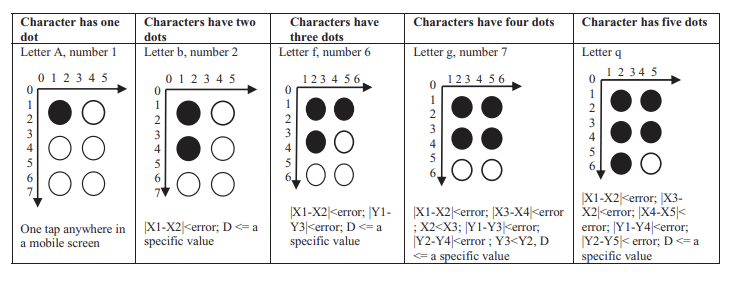
\includegraphics{ch02/assets/categorization-of-braille.png}
    \decoRule
    \caption[Categorização de coordenadas do SingleTapBraille]{Amostra de categorização de caracteres braille com base no número de pontos \parencite{REF07}}
    \label{fig:ch02-categorization-of-braille}
\end{figure}

O principal conceito por trás do método de entrada é o agrupamento de pontos braille ativados para cada caractere. Quando o usuário para de tocar na tela por um curto intervalo, nosso algoritmo agrupa os toques inseridos e os interpreta com base no número de pontos. O algoritmo processa as coordenadas de cada ponto, bem como o espaço entre cada ponto e o seguinte.

A principal vantagem é que não restringe os usuários, exigindo que encontrem um objeto específico na tela, em vez disso, permite que eles toquem nos pontos braille em qualquer lugar da tela com base em padrões braille. Não possui botão ou outro tipo de controle que exija que o usuário toque ou clique com precisão em pontos específicos. É totalmente acionado por gestos e possui uma saída de voz correspondente. 

É importante ressaltar que a aplicação pode ser usada tanto por pessoas estacionárias quanto por pessoas em movimento. Existem algumas operações de digitação, como espaço e backspace, que o teclado braille não apresenta utilizando pontos braille, pois possuem botões específicos na máquina braille que realizam essas funções, e que foi simulado através de gestos do usuário.

\begin{figure}[h]
    \centering
    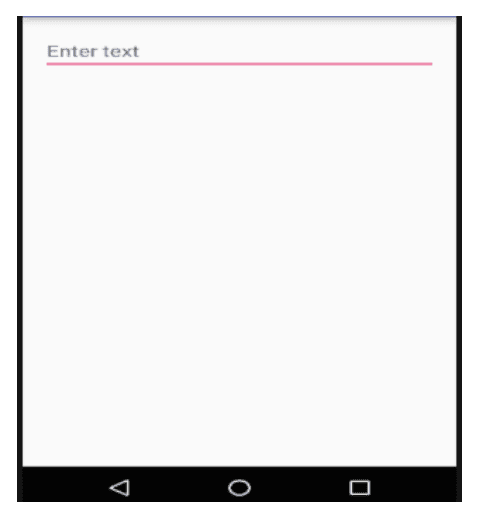
\includegraphics[scale=0.5]{ch02/assets/singletapbraille-gui.png}
    \decoRule
    \caption[Interface do SingleTapBraille]{Interface do SingleTapBraille \parencite{REF07}}
    \label{fig:ch02-singletapbraille-gui}
\end{figure}

O SingleTapBraille foi projetado para usuários que conhecem braille e sabem ler e escrever em braille, além de terem experiência com dispositivos touchscreen. Esta aplicação tem como objetivo melhorar a velocidade de digitação e edição na tela do celular, ao mesmo tempo que minimiza a taxa de erros.

\subsection{Brailendo}

O Brailendo \parencite{REF09} é uma ferramenta criada com o propósito de auxiliar alunos e professores a aprenderem e praticarem de forma autônoma o Sistema Braille em suas várias representações do Braille, como textual, matemático, musical, entre outros.

Em sua interface principal, é possível digitar normalmente no teclado, e a medida que o usuário digita aparece as células equivalentes em Braille, assim como os pontos em forma de números, e o texto em metabraille.

Nessa mesma interface, o Braillendo dá a possibilidade de digitar usando as teclas 'F', 'D', 'S', 'J', 'K', 'L' do teclado computador do usuário, simulando o uso de uma Máquina Braille real.

\begin{figure}[h]
    \centering
    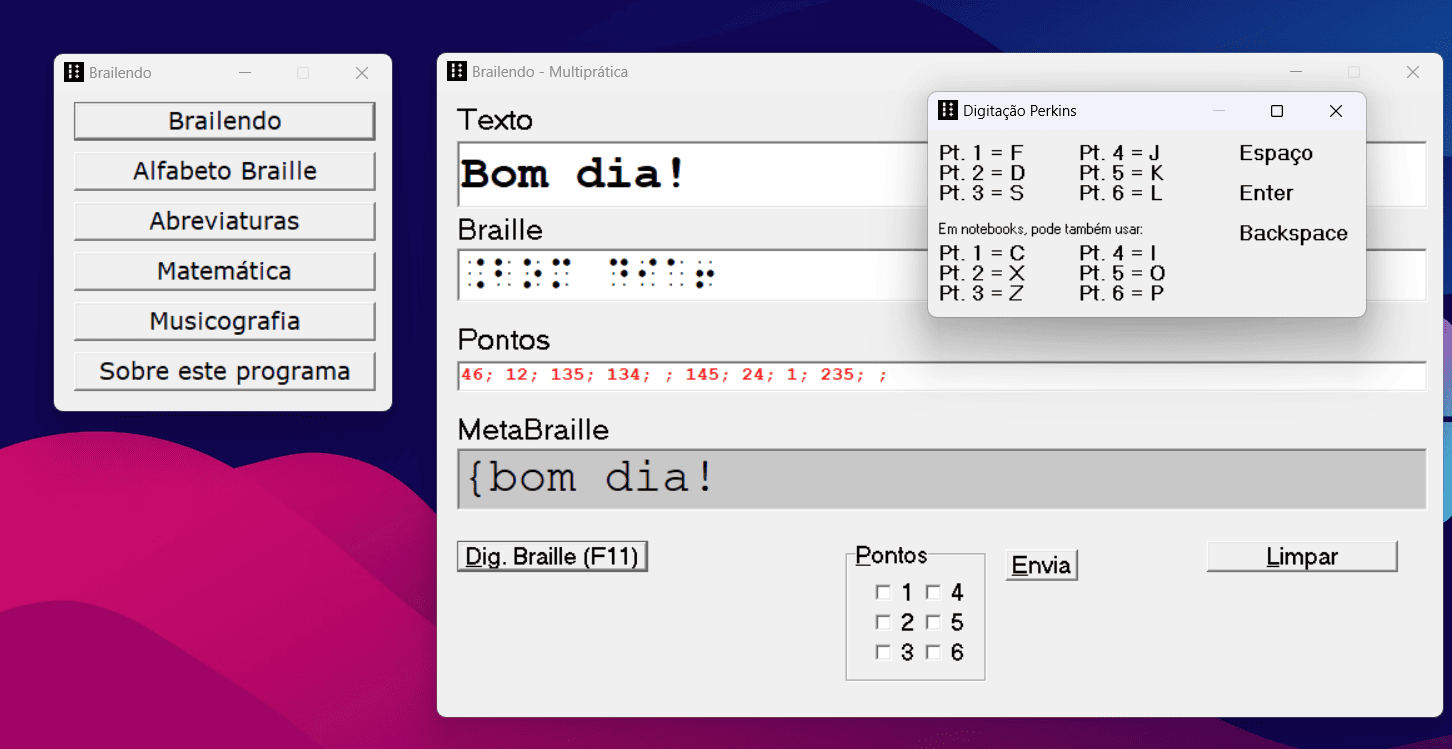
\includegraphics[scale=0.3]{ch02/assets/brailendo-gui.png}
    \decoRule
    \caption[Interface do Brailendo]{Interface do Brailendo}
    \label{fig:ch02-brailendo-gui}
\end{figure}

Além disso, a aplicação disponibiliza várias outras interfaces que contém todas células Braille, funções que permitem aprender e praticar a mecânica de criação de expressões matemáticas em braille, funções que permitem a conversão direta entre expressões escritas em asciiMath e braille, além de uma opção de musicografia em braille, onde aparece um teclado virtual, e ao selecionar as teclas, aparece a representação em notas musicais e também em Braille. É possível reproduzir o som após escolher uma combinação de notas musicais.

\subsection{Braillearning}

O Braillearnig \parencite{REF08} foi desenvolvido para auxiliar pessoas com deficiência visual no uso e aprendizado da Máquina Braille, além de ajudá-los na memorização do alfabeto Braille, sendo esse software um alternativa gratuita à Máquina Braille.

Para simular os botões da Máquina Braille, o Braillearning utiliza as teclas 'F', 'D', 'S', 'J', 'K', 'L' do teclado computador do usuário, simulando as teclas que representam os pontos 1, 2, 3, 4, 5 e 6 na máquina física. Assim, a ferramenta simula o uso real de uma Máquina Braille. O resultado da combinação de teclas pressionadas é exibido na tela com a letra, número ou símbolo equivalente no texto a tinta.

\begin{figure}[h]
    \centering
    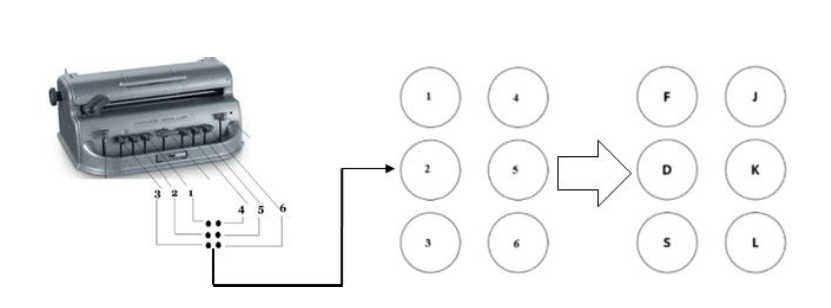
\includegraphics[scale=0.5]{ch02/assets/braillearning-keys.png}
    \decoRule
    \caption[Teclas do Braillearning]{Máquina de escrever em Braille e teclas utilizadas no Braillearning \parencite{REF08}}
    \label{fig:ch02-braillearning-modes}
\end{figure}

O Braillearning possui três modos de uso: tutorial, palavra e livre.

No modo tutorial o usuário recebe em formato de áudio e imagem um caractere, e então o usuário tem que pressionar as teclas que formam o caractere equivalente em Braille. Este modo é focado no aprendizado do Braille, por isso, oferece atalhos para dicas, no caso do usuário precisar.

O modo palavra sorteia uma palavra e a exibe, o usuário então deve digitar essa palavra usando a simulação das teclas da Máquina Braille. Enquanto o usuário vai acertando ele recebe como saída o caractere digitado e um efeito sonoro de sucesso. No caso de erro, um efeito sonoro de erro é reproduzido ao usuário, e então ele pode tentar novamente fazer a combinação de letras.

O modo livre permite ao usuário digitar livremente o que ele quiser no simulador. É o modo que mais se assemelha ao uso real da Máquina Braille.

Após os Braillearning se mostrou uma ferramenta que simula bem o uso real da Máquina Braille, podendo ser utilizada tanto por usuários videntes quanto por usuários com deficiência visual. O simulador pode ser usuado tanto para aprendizado do Braille e Máquina Braille, quando para apenas praticar o seu uso.

\begin{figure}[h]
    \centering
    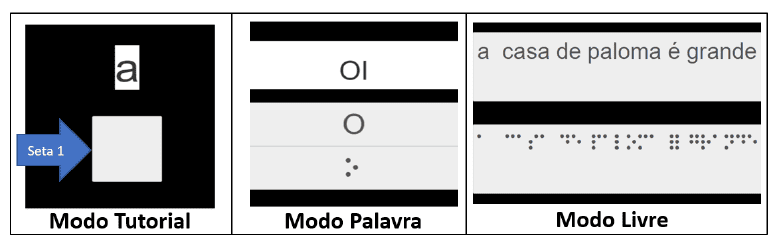
\includegraphics[scale=0.5]{ch02/assets/braillearning-modes.png}
    \decoRule
    \caption[Modos do Braillearning]{Modos de operação do Braillearning \parencite{REF08}}
    \label{fig:ch02-braillearning-modes}
\end{figure}

Apesar da semelhança, o contato com a Máquina Braille real continua sendo indispensável, visto que é necessário a prática da leitura do Braille com as mãos, o que não é possível com o Braillearning, sendo possível apenas a leitura com os outros ou ouvindo os leitores de tela.

\subsection{Braille Fácil}

O Braille Fácil \parencite{REF09} é uma ferramenta criada para facilitar e agilizar a criação de uma impressão em Braille. O texto a ser impresso pode ser digitado diretamente na aplicação ou pode ser importado a partir de um arquivo de texto simples. Com o texto na aplicação, o usuário pode visualizar com será a impressão. 

O Braille Fácil se encarrega de converter cada caractere para os sinal Braille equivalente. O programa gera arquivos de impressão com compatibilidade para diversas impressoras. Além de agilizar o processo de geração de números de páginas, gráficos e controle de margens.

\begin{figure}[h]
    \centering
    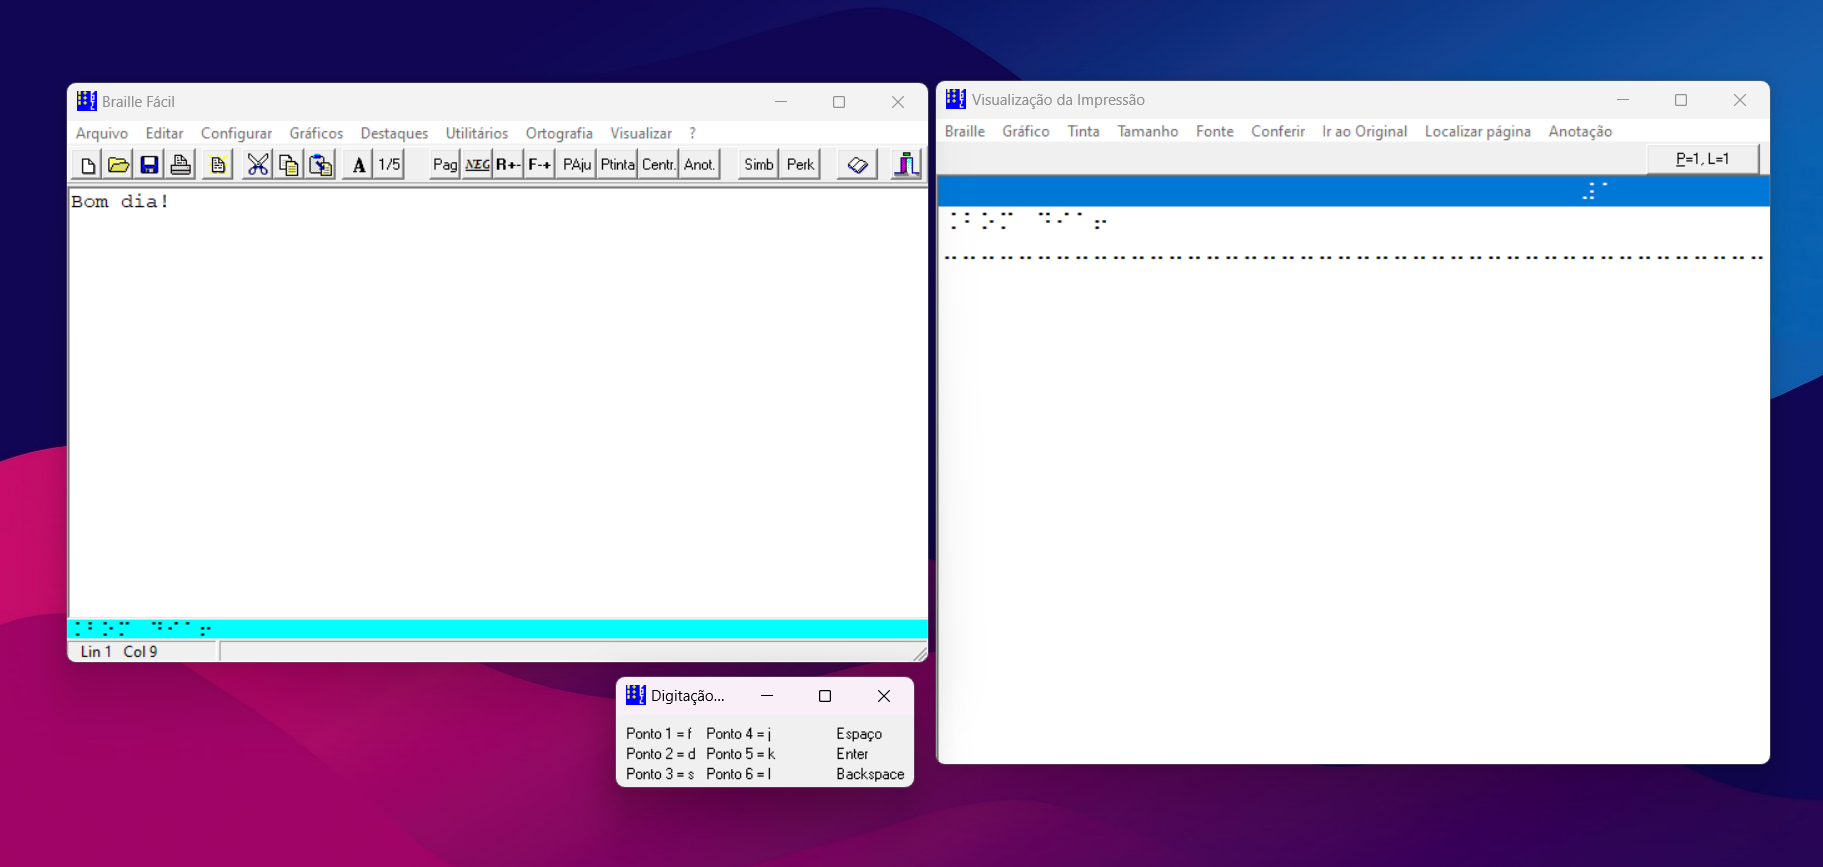
\includegraphics[scale=0.3]{ch02/assets/braille-facil-gui.png}
    \decoRule
    \caption[Interface do Braille Fácil]{Interface do do Braille Fácil}
    \label{fig:ch02-braille-facil-gui}
\end{figure}

Também dispõe de uma funcionalidade de escrita simulando uma Máquina Braille utilizando as teclas 'F', 'D', 'S', 'J', 'K', 'L' do teclado computador. Assim, um usuário cego pode digitar na aplicação como se estivesse usando uma Máquina Braille real.

\section{Aplicações Simuladoras da Máquina Braille}

\subsection{Duxbury Systems: Perky Duck}

A aplicação Perky Duck é uma ferramenta que simula a funcionalidade de uma máquina braille, facilitando a produção de documentos acessíveis para pessoas com deficiência visual. Desenvolvido pela Duxbury Systems, o Perky Duck é uma extensão do popular software de editoração Duxbury Braille Translator (DBT), e sua funcionalidade principal reside na emulação da máquina braille. 

\begin{figure}[h]
    \centering
    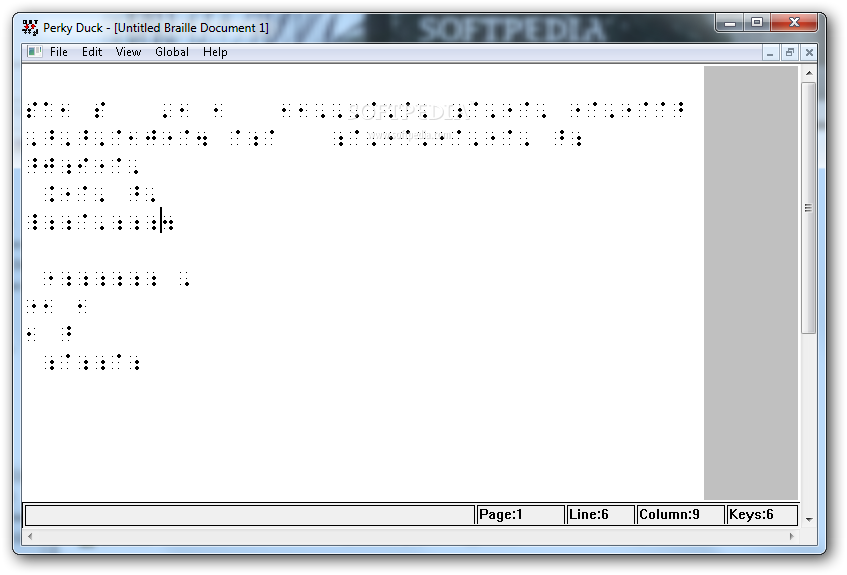
\includegraphics[scale=0.5]{ch02/assets/perky-duck-gui.png}
    \decoRule
    \caption[Interface do Perky Duck]{Interface do Perky Duck}
    \label{fig:ch02-perky-duck-gui}
\end{figure}

Disponível para Windows e MAC OS, a aplicação replica as características táteis da máquina braille, permitindo que os usuários experimentem virtualmente o processo de criação de documentos em braille. Para garantir uma experiência inclusiva, o Perky Duck fornece feedback auditivo e visual durante o uso. Isso inclui sons indicativos de progresso, juntamente com visualização na tela para acompanhar a tradução de texto para braille. 

Os usuários podem selecionar diferentes tipos de braille, ajustar o espaçamento entre células, definir configurações de formatação e entre outros, para atender às suas preferências individuais e requisitos específicos.

\subsection{Accessibyte: Braillio}

Braillio é uma aplicação web paga, projetada para auxiliar no aprendizado de Braille e da Máquina Braille. A aplicação pode ser acessada através de dispositivos móveis.

Uma característica central da aplicação é a simulação tátil e sonora da máquina Braille. Ao interagir com a aplicação, os usuários experimentam a sensação realista de pressionar as teclas da máquina Braille, acompanhada por sons que imitam o mecanismo de impressão. Isso proporciona uma experiência imersiva que ajuda os usuários a entender e memorizar a disposição dos pontos Braille. Os usuários recebem pistas auditivas, feedback tátil através de vibrações na tela (se estiverem usando um dispositivo touchscreen) e prompts visuais para reforçar sua compreensão dos caracteres e padrões Braille. Essa abordagem multissensorial atende a diferentes estilos de aprendizado e promove a retenção.

\begin{figure}[h]
    \centering
    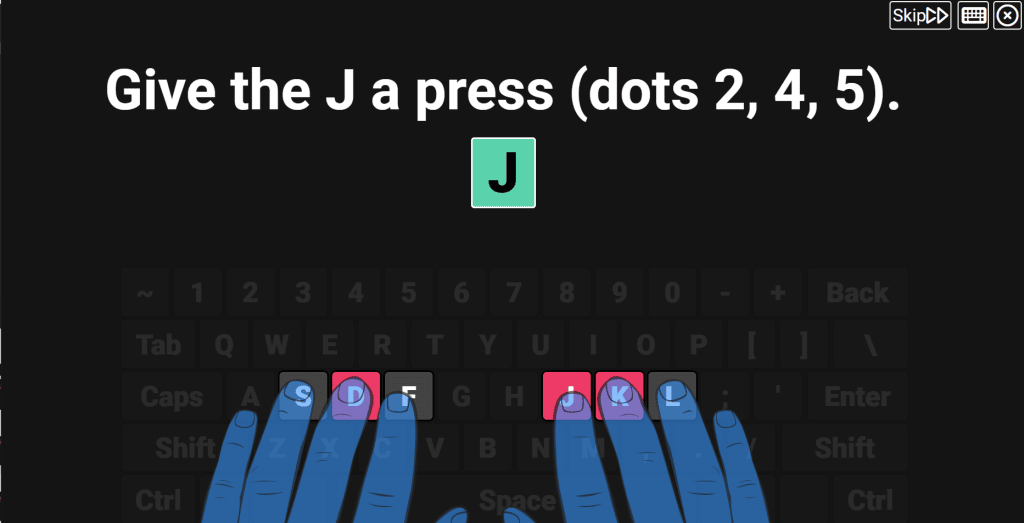
\includegraphics[scale=0.3]{ch02/assets/braillio-gui.png}
    \decoRule
    \caption[Interface do Braillio]{Interface do Braillio}
    \label{fig:ch02-braillio-gui}
\end{figure}

O Braillio oferece uma série de lições interativas que guiam os usuários pelos fundamentos do Braille. Essas lições são cuidadosamente estruturadas para introduzir gradualmente o alfabeto Braille, contrações, pontuação e mais. Cada lição incorpora instruções de áudio, feedback tátil e exercícios interativos para reforçar a aprendizagem. Com uma interface intuitiva e fácil de usar, torna a prática do Braille acessível a iniciantes e usuários avançados. 

Os usuários podem praticar a digitação de caracteres individuais, palavras e frases completas, recebendo feedback instantâneo sobre sua precisão e velocidade. Isso facilita a prática regular e o aprimoramento das habilidades em Braille.


\section{Desafios e Oportunidades}

Garantir que a simulação da máquina de escrever em Braille seja fiel à experiência real é um grande desafio a se enfrentar. Isso inclui replicar com precisão as sensações táteis e sonoras associadas ao uso da máquina, garantindo uma experiência imersiva e autêntica para os usuários. Embora deva oferecer um feedback auditivo e visual durante o uso, garantir a acessibilidade para usuários com diferentes necessidades sensoriais pode ser difícil. Isso inclui fornecer opções para usuários surdos ou com deficiência auditiva, bem como aqueles com limitações visuais.

Os simuladores precisam atender às necessidades de uma ampla gama de usuários, desde iniciantes no Braille até usuários avançados. Isso requer a implementação de recursos que sejam intuitivos para iniciantes, mas também desafiadores e personalizáveis para usuários mais experientes. Além de oferecer lições e exercícios que guiem os usuários desde os fundamentos básicos até habilidades mais avançadas, garantindo uma curva de aprendizado suave e eficiente.

Com o advento da tecnologia web, os simuladores podem ser acessados em uma variedade de dispositivos, incluindo computadores, tablets e smartphones. Isso aumenta sua acessibilidade global, permitindo que mais pessoas em diferentes contextos e localizações geográficas acessem as ferramentas de aprendizado do Braille. Podendo servir como plataformas para colaboração e comunidade, permitindo que os usuários compartilhem recursos, dicas e experiências de aprendizado. Isso cria um ambiente de apoio e colaboração entre os aprendizes de Braille, promovendo uma abordagem de aprendizado social e engajada.

\section{Comparativo entre aplicações}

% Após análise das aplicações vemos que em sua maioria são aplicações gratuitas. Porém apenas duas são web, as outras aplicação são da plataforma Android, Windows ou MAC. O problema de 

As aplicações existentes, como o BrailleType, SingleTapBraille, Brailendo, Braillearning, Perky Duck e Braillio, abordam diferentes aspectos do aprendizado e prática do Braille, cada uma com suas particularidades e limitações. O BrailleType e o SingleTapBraille focam em interfaces touchscreen, com uma abordagem simples e acessível para usuários com dispositivos móveis, porém, com uma ênfase maior no uso de um dedo ou polegar e menor semelhança com a Máquina Braille real. O Brailendo e o Braillearning oferecem simulações mais próximas da experiência com a Máquina Braille, utilizando o teclado físico, e são boas alternativas para o aprendizado prático, mas a interação ainda se limita a modos tutoriais ou específicos, sem tanta flexibilidade para aprendizado independente ou desafios. O Perky Duck e o Braillio, por sua vez, são mais focados na produção de documentos em Braille, com uma ênfase maior na criação de arquivos e personalização de formatos. Diante desse cenário, o projeto proposto se destaca ao oferecer uma solução gratuita e acessível, simulando de maneira fiel a experiência da Máquina Braille com o uso do teclado físico, proporcionando uma transição mais fluida para o uso real da máquina. Além disso, a aplicação inclui um Modo de Desafio interativo, que promove um ambiente dinâmico de prática e aprendizado, com feedback auditivo e visual, facilitando o ensino do Braille e a prática da Máquina Braille de forma mais acessível e imersiva, contribuindo significativamente para a inclusão e autonomia de pessoas com deficiência visual.

\begin{table}[h]
    \caption{Comparativo de aplicações}
    \label{tab:ch02-comparative}
    \centering
    \begin{tabular}{llcc}
        \toprule
        \tabhead{Aplicação}&  \tabhead{Plataforma}&  \tabhead{É gratuita?}& \tabhead{Ensina Braille?}\\
        \midrule
        BrailleType&  Android&  Sim& Não\\
        \addlinespace
        SingleTapBraille&  Android&  Sim& Não\\
        \addlinespace
        Brailendo&  Windows&  Sim& Sim\\
        \addlinespace
        Braillearnig&  Windows&  Sim& Sim\\
        \addlinespace
        Braille Fácil&  Windows&  Sim& Não\\
        \addlinespace
        Perky Duck&  Windows e MAC&  Sim& Não\\
        \addlinespace
        Braillio&  Web&  Não& Sim\\
        \addlinespace
        SWBraille& Web& Sim&Sim\\
        \bottomrule\\
    \end{tabular}
\end{table}


\chapter{Análise de Valor} 
\label{chap:Chapter03} 

\section{Processo de Inovação}

\subsection{Conceito de Processo de Inovação}

O processo de inovação pode ser dividido em três áreas principais: o Fuzzy Front End (FFE), o Processo de Desenvolvimento de Novos Produtos (DNP) e a comercialização \parencite{BOOK01}. Cada uma dessas áreas desempenha um papel no ciclo de inovação, contribuindo para transformar ideias em produtos, serviços ou processos que geram valor para a organização e seus clientes. 

A primeira parte, Fuzzy Front End, é geralmente considerada uma das mais importantes para a melhoria do processo de inovação \parencite{BOOK01}. Essa fase inicial é caracterizada pela sua natureza incerta e exploratória, onde novas oportunidades de mercado são identificadas e um grande número de ideias é gerado e refinado.

Nesse capítulo, a atenção será voltada para as atividades do Fuzzy Front End, que têm objetivo de aumentar o valor, a quantidade e a probabilidade de sucesso dos conceitos lucrativos que entram nas fases posteriores de desenvolvimento e comercialização de produtos. Exploraremos práticas para identificar oportunidades promissoras, métodos eficazes para gerar e enriquecer ideias e estratégias para selecionar os conceitos mais viáveis.

\begin{figure}[h]
    \centering
    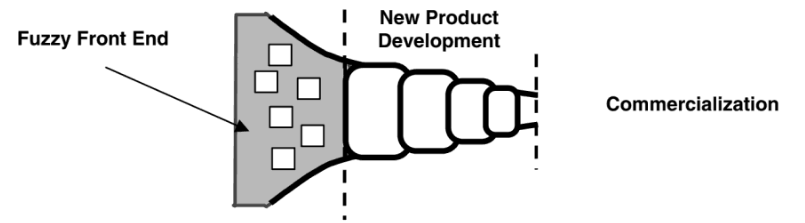
\includegraphics[scale=0.5]{ch03/assets/inovation-process.png}
    \decoRule
    \caption[Processo de Inovação]{Processo de Inovação \parencite{BOOK01}}
    \label{fig:ch02-inovation-process}
\end{figure}

\subsection{New Concept Development (NCD)}

O modelo \textit{New Concept Development} (NCD) é composto por três partes principais \parencite{BOOK01}:

\begin{itemize}
    \item \textbf{Parte central ou motor:} Consiste na liderança, cultura e estratégia de negócios da organização, que impulsionam os cinco elementos-chave controláveis pela empresa.
    
    \item \textbf{Área interna de raios:} Define os cinco elementos de atividade controláveis do Fuzzy Front End (FFE), que são: 
    \begin{itemize}
        \item Identificação de oportunidades
        \item Análise de oportunidades
        \item Geração e enriquecimento de ideias
        \item Seleção de ideias
        \item Definição de conceito
    \end{itemize}

    \item \textbf{Fatores de influência:} Incluem as capacidades organizacionais, o ambiente externo (como canais de distribuição, legislação, políticas governamentais, clientes, concorrentes e o clima político e econômico) e as ciências facilitadoras (tanto internas quanto externas). Esses fatores influenciam todo o processo de inovação até a comercialização e são relativamente incontroláveis pela empresa.
\end{itemize}

\begin{figure}[h]
    \centering
    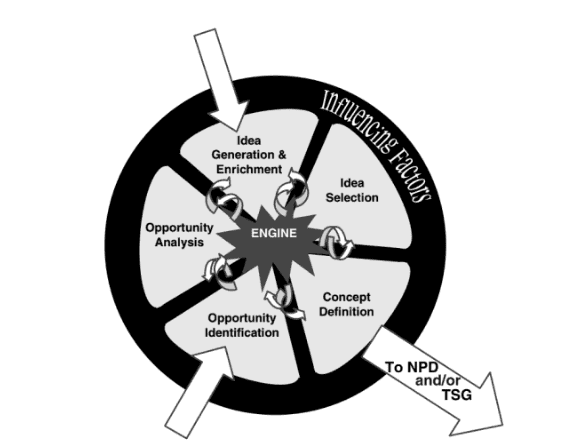
\includegraphics[scale=0.5]{ch03/assets/new-concept-development.png}
    \decoRule
    \caption[New Concept Development]{New Concept Development \parencite{BOOK01}}
    \label{fig:ch02-inovation-process}
\end{figure}

\subsection{Identificação da oportunidade}

Nessa atividade, se busca identificar oportunidades que possam ser exploradas para impulsionar o crescimento e eficiência \parencite{BOOK01}. Essa oportunidade pode representar uma nova direção para o negócio ou uma atualização de produtos existentes. Pode incluir o desenvolvimento de novas plataformas de produtos, processos de fabricação, ofertas de serviços ou abordagens de marketing e vendas. A identificação inicial da oportunidade define o mercado ou a área tecnológica na qual a solução irá se envolver.

A necessidade de desenvolver soluções acessíveis para o aprendizado do Braille é evidenciada pela alta demanda e os altos custos das Máquinas de escrever em Braille, como descrito em na seção \ref{sec:ch02_Valores_da_Maquina_Braille}. Pessoas com deficiência visual, especialmente aquelas que ficaram cegas recentemente, enfrentam barreiras significativas no acesso a essas ferramentas essenciais. Instituições educacionais e organizações dedicadas ao suporte de pessoas com deficiência visual também enfrentam desafios devido à necessidade de múltiplas máquinas para práticas em grupo. 

Portanto, a oportunidade reside em criar uma ferramenta virtual que possa preencher essa lacuna, proporcionando um ambiente de aprendizado eficaz e acessível.

\subsection{Análise da oportunidade}

Essa atividade envolve a identificação e avaliação de potenciais oportunidades de mercado, necessidades dos clientes, tendências tecnológicas e lacunas no mercado \parencite{BOOK01}. Nesta fase as informações podem ser incertas, ambíguas ou incompletas, o que significa que a análise de oportunidades pode ser desafiadora. A análise de oportunidades no Fuzzy Front End pode incluir técnicas como pesquisa de mercado, análise de tendências, brainstorming, análise SWOT (Strengths, Weaknesses, Opportunities, Threats), análise de cenários, entre outros métodos para identificar e entender as oportunidades que podem guiar o desenvolvimento de novos produtos ou serviços \parencite{BOOK01}. Nessa seção usaremos a técnica de análise SWOT.

Os principais beneficiários desta aplicação são pessoas com deficiência visual, educadores e instituições que oferecem suporte a essas pessoas. Esses usuários precisam de uma solução prática, acessível e eficaz para o aprendizado do Braille. A aplicação web deve ser intuitiva e replicar a experiência de usar uma Máquina de escrever em Braille, permitindo que os usuários pratiquem de forma realista. Além disso, deve oferecer feedback sonoro e visual para auxiliar no processo de aprendizado.

\begin{figure}[h]
    \centering
    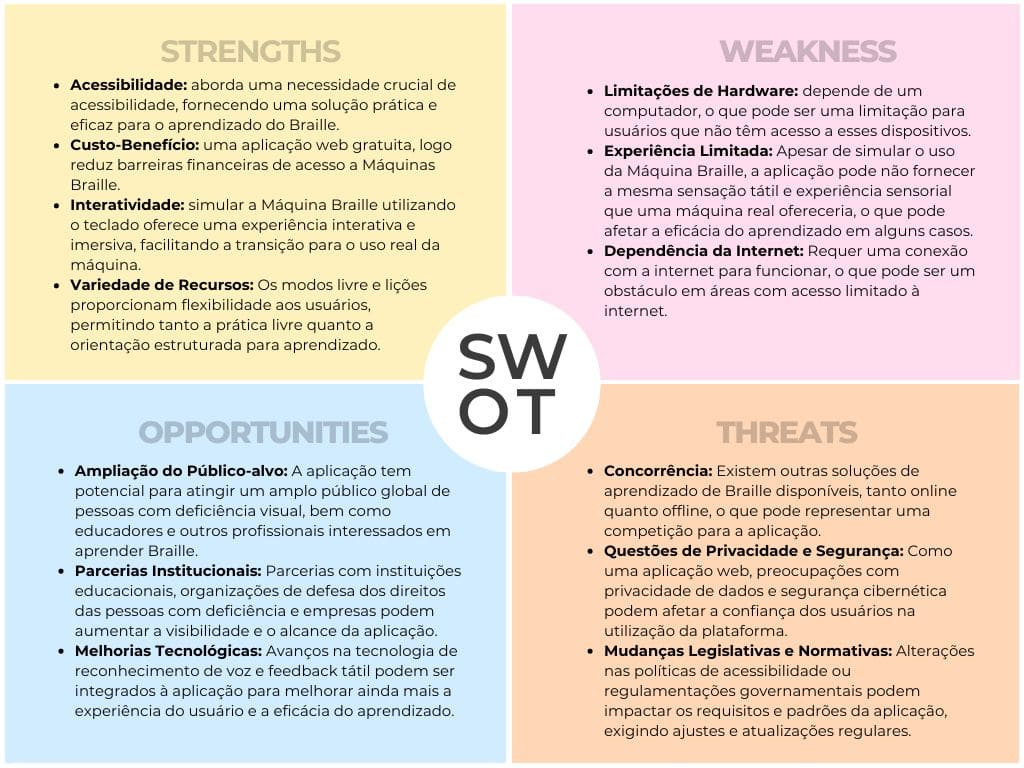
\includegraphics[scale=0.4]{ch03/assets/analise-swot.jpg}
    \decoRule
    \caption[Análise SWOT]{Análise SWOT}
    \label{fig:ch02-analise-swot}
\end{figure}

Inicialmente, as forças do projeto são notáveis. A acessibilidade é uma vantagem crucial, pois aborda uma necessidade significativa para pessoas com deficiência visual, fornecendo uma solução prática e gratuita para o aprendizado do Braille. Além disso, a interatividade oferecida pela aplicação, juntamente com sua variedade de recursos, como os modos de Modo Livre e Modo de Lições, promove uma experiência flexível e envolvente para os usuários.

No entanto, a aplicação possui algumas fraquezas a serem consideradas. A dependência do acesso a um computador pode excluir potenciais usuários que não têm acesso a esses dispositivos, enquanto a falta de sensação tátil pode limitar a experiência de aprendizado em comparação com o uso de uma máquina real. Além disso, a necessidade de uma conexão estável com a internet pode ser uma limitação em áreas com acesso limitado à rede.

Por outro lado, contém diversas oportunidades para ampliar seu impacto e alcance. Com potencial para atingir um amplo público global e estabelecer parcerias com instituições educacionais e organizações de defesa dos direitos das pessoas com deficiência, a aplicação pode expandir sua influência e utilidade. Além disso, a integração de melhorias tecnológicas, como reconhecimento de voz e feedback tátil, pode aprimorar ainda mais a experiência do usuário.

No entanto, o projeto também enfrenta ameaças, como a concorrência de outras soluções de aprendizado de Braille e preocupações com privacidade de dados e segurança cibernética. Mudanças nas políticas de acessibilidade ou regulamentações governamentais também podem representar desafios futuros que exigem adaptação e flexibilidade.

Em suma, embora o projeto apresente desafios significativos, suas forças e oportunidades superam essas limitações, o posicionando como uma ferramenta valiosa para promover a inclusão e a autonomia de pessoas com deficiência visual. Com uma abordagem estratégica e contínua inovação, o projeto tem o potencial de fazer uma diferença positiva na vida de muitos indivíduos.

\subsection{Geração e enriquecimento de ideias}

Nessas atividade é abordado o processo de concepção, desenvolvimento e refinamento de uma ideia concreta \parencite{BOOK01}. Esse processo é altamente iterativo e evolutivo, envolvendo a construção, destruição, combinação, remodelação, modificação e atualização de ideias. As ideias passam por diversas iterações e mudanças à medida que são exploradas, estudadas, discutidas e desenvolvidas em conjunto com outros elementos do modelo de Desenvolvimento de Novos Produtos \parencite{BOOK01}.

As principais funcionalidades da aplicação foram determinadas com base nas necessidades dos usuários:

\begin{itemize}
    \item \textbf{Simulação das teclas da Máquina Braille:} Utilização das teclas F, D, S, J, K e L para simular os pontos do Braille.
    \item \textbf{Feedback Sonoro:} Cada caractere escrito deve ser acompanhado por um feedback sonoro.
    \item \textbf{Modos de Uso:} Um Modo Livre para prática livre e um Modo de Lições com exercícios estruturados.
    \item \textbf{Visualização do Texto}: Exibição do texto em Braille e em tinta para facilitar o entendimento dos usuários.
    \item \textbf{Navegação:} Uso das setas do teclado para navegar pelo texto.
\end{itemize}

\subsection{Seleção da ideia}

A seleção de ideias envolve uma série iterativa de atividades, que incluem múltiplas revisões da identificação de oportunidades, análise de oportunidades e geração e enriquecimento de ideias \parencite{BOOK01}. 

Durante a fase de geração de ideias, diversas propostas foram consideradas para o desenvolvimento da aplicação simuladora da Máquina de escrever em Braille. Cada ideia foi avaliada com base em sua capacidade de atender às necessidades dos usuários e oferecer uma solução acessível, prática e eficaz para o aprendizado e prática do Braille. Após análise, todas as ideias foram selecionadas para compor o conceito final da aplicação.

Cada uma dessas ideias foi considerada crucial para o desenvolvimento de uma aplicação web simuladora da Máquina de escrever em Braille que seja acessível, prática e eficaz. A combinação dessas funcionalidades proporcionará uma experiência completa e satisfatória para os usuários, contribuindo assim para a promoção da inclusão e autonomia de pessoas com deficiência visual.

\subsection{Definição do conceito}

A definição do conceito é a última atividade no novo modelo de desenvolvimento de produtos. Nesse estágio, o inovador precisa convencer os responsáveis pela decisão a investirem na proposta de negócio ou tecnologia. Isso é muitas vezes chamado de "declaração de vitória" ou "documento de entrada". Geralmente, são considerados objetivos, tamanho da oportunidade ou até mesmo necessidades do mercado ou do cliente \parencite{BOOK01}.

O conceito para a aplicação foi definido para atender às necessidades dos usuários e proporcionar uma solução acessível, prática e eficaz para o aprendizado e prática do Braille. Através da análise das ideias geradas e da seleção das funcionalidades mais relevantes, o conceito final da aplicação é por vários pontos.

\subsubsection{Simulação Precisa da Máquina Braille}

A aplicação irá mapear as teclas do teclado do computador para simular os pontos do Braille, garantindo uma representação fiel da Máquina Braille real. Cada tecla correspondente aos pontos do Braille será atribuída a uma tecla específica do teclado, proporcionando uma experiência autêntica para os usuários.

\subsubsection{Feedback Multissensorial}

Será fornecido feedback sonoro e visual para cada caractere digitado. Quando uma tecla for pressionada, um som específico será reproduzido, indicando o caractere correspondente. Além disso, o caractere será exibido na tela em formato Braille, permitindo que os usuários visualizem o resultado de sua entrada.

\subsubsection{Modos de Uso Versáteis}

A aplicação oferecerá diferentes modos de uso para atender às necessidades dos usuários. No Modo Livre, os usuários podem praticar livremente, digitando textos e explorando a funcionalidade da Máquina Braille. No Modo de Lições, serão disponibilizados exercícios estruturados para facilitar o aprendizado do Braille, guiando os usuários por meio de atividades interativas.

\subsubsection{Visualização do Texto em Braille e em Tinta}

O texto digitado será apresentado tanto em Braille quanto em tinta, permitindo que os usuários visualizem o conteúdo de forma acessível. Essa funcionalidade visa atender às necessidades de usuários menos familiarizados com o Braille, facilitando sua compreensão do texto.


\section{Valor da solução}

\subsection{Valor}

O conceito de valor, especialmente no contexto de marketing, é essencial para entender a lealdade e satisfação do cliente \parencite{BOOK02}. Diversos autores ofereceram definições e perspectivas distintas sobre o que constitui valor. \textcite{BOOK03} define valor como uma crença duradoura na preferência por um modo de conduta ou estado final específico em detrimento de outro. \textcite{ARTICLE10}, por sua vez, apresenta três definições: valor como preço baixo, como a qualidade recebida pelo preço pago e como o trade-off entre o que se recebe e o que se dá. Esta última definição é complementada por \textcite{BOOK04}, que também destacam o trade-off entre a qualidade do item e seus custos.

Desenvolvendo ainda mais a noção de trade-off, \textcite{BOOK05} define valor como a diferença entre os benefícios percebidos e os sacrifícios percebidos pelos clientes. Benefícios percebidos podem incluir qualidade do produto, serviço associado, benefícios relacionais e de imagem, enquanto os sacrifícios incluem custos monetários, de tempo, energia e psicológicos. \textcite{BOOK06} ampliam essa definição, considerando o valor como a soma dos benefícios técnicos, econômicos, de serviço e sociais que um cliente recebe em troca do preço pago. Esta abordagem destaca que o valor é uma avaliação subjetiva do cliente, baseada na percepção dos benefícios recebidos em comparação com os custos incorridos.

Finalmente, é importante reconhecer que o conceito de valor pode variar conforme a perspectiva do cliente. \textcite{ARTICLE11} observa que as percepções de “o que é recebido” e “o que é dado” variam de cliente para cliente, enfatizando que o valor é um trade-off entre esses componentes. Em termos práticos, muitas vezes os proprietários de negócios, resumem valor na simples máxima "você recebe o que paga", refletindo a inter-relação entre preço, qualidade e satisfação do cliente. Assim, compreender o valor de maneira holística e adaptada às percepções dos clientes é crucial para as estratégias de marketing e fidelização.

\subsection{Valor do produto}

\textcite{ARTICLE10} afirma que o conceito de valor do produto para o cliente (\textit{perceived value}) varia entre os consumidores, refletindo suas percepções pessoais. Entrevistados utilizam o termo "valor" de maneiras diversas, abrangendo uma ampla gama de atributos e abstrações. Esse valor é altamente subjetivo e pode ser definido de quatro formas principais: 

\begin{enumerate}
    \item \textbf{Valor é preço baixo}, onde o custo é o fator predominante;
    \item \textbf{Valor é tudo o que quero em um produto}, enfatizando a satisfação dos desejos e utilidades individuais;
    \item \textbf{Valor é a qualidade que obtenho pelo preço que pago}, onde a troca justa entre preço e qualidade é crucial;
    \item \textbf{Valor é o que recebo pelo o que dou}, considerando um equilíbrio entre todos os benefícios recebidos e os custos suportados.
\end{enumerate}

Essas definições demonstram a complexidade de conceituar e medir o valor percebido na pesquisa de marketing. Enquanto alguns consumidores focam principalmente no aspecto monetário, outros dão mais importância aos benefícios e conveniências que o produto oferece. Há também aqueles que veem valor como uma troca equilibrada entre preço e qualidade, e outros que consideram todos os aspectos de dar e receber na sua avaliação de valor \parencite{ARTICLE10}.

Segundo \textcite{ARTICLE10}, a perspectiva longitudinal do valor do produto para o cliente pode ser segmentada em quatro fases principais: 

\begin{itemize}
    \item Antes da compra;
    \item Na aquisição;
    \item Após a compra;
    \item Após o uso ou experiência.
\end{itemize}

No estágio pré-compra, o valor é percebido através do "valor desejado" e "valor esperado", onde os clientes formam expectativas sobre os benefícios que esperam obter e os sacrifícios que estão dispostos a fazer \parencite{ARTICLE10}. Durante a aquisição, o valor é experimentado em tempo real como "valor de transação" e "valor de aquisição", refletindo a avaliação imediata dos benefícios recebidos contra os sacrifícios feitos, como o custo e o esforço da compra \parencite{ARTICLE10}. Após a compra, o valor se manifesta como "valor entregue", "valor recebido', "valor de uso' e "valor pós-compra/desempenho", onde os clientes avaliam os benefícios contínuos e a utilidade do produto ou serviço, considerando os sacrifícios já realizados \parencite{ARTICLE10}. Finalmente, após o uso ou experiência, o valor é percebido como "valor de resgate", considerando os benefícios remanescentes ou o valor residual no ponto de disposição ou revenda, contrastando com os sacrifícios iniciais e contínuos feitos \parencite{ARTICLE10}. 

\begin{figure}[h]
    \centering
    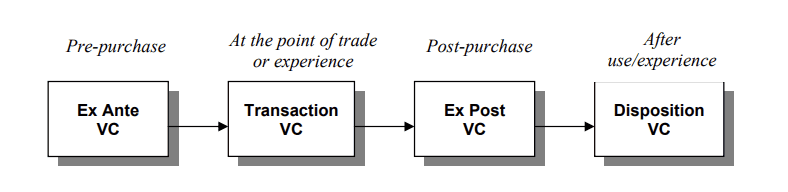
\includegraphics[scale=0.7]{ch03/assets/longitudinal-perspective.png}
    \decoRule
    \caption[Perspectiva longitudinal do valor do produto para o cliente]{Perspectiva longitudinal do valor do produto para o cliente \parencite{ARTICLE10}}
    \label{fig:ch02-longitudinal-perspective}
\end{figure}

Essa estrutura longitudinal revela como o valor do produto para o cliente evolui ao longo do tempo, influenciando as percepções de benefícios e sacrifícios dos clientes em diferentes etapas de sua jornada.

\subsubsection{Antes da Compra}

\textbf{Benefícios:}

\begin{itemize}
    \item \textbf{Acessibilidade:} A aplicação web é gratuita e disponível online, eliminando a barreira financeira que impede o acesso às máquinas Braille físicas.
    \item \textbf{Praticidade:} Permite o aprendizado e prática do Braille em qualquer lugar com acesso a um computador, sem a necessidade de equipamento especializado.
    \item \textbf{Inclusão:} Oferece uma solução inclusiva que pode ser usada por pessoas recém-deficientes visuais e por educadores em ambientes de ensino inclusivo.
\end{itemize}

\textbf{Sacrifícios:}

\begin{itemize}
    \item \textbf{Necessidade de Recursos:} O usuário precisa ter acesso a um computador com teclado físico e conexão à internet.
    \item \textbf{Curva de Aprendizado Inicial:} Usuários que não estão familiarizados com o uso de computadores podem encontrar dificuldades iniciais.
\end{itemize}

\subsubsection{Na Aquisição}

\textbf{Benefícios:}

\begin{itemize}
    \item \textbf{Imediata Disponibilidade:} A aplicação pode ser acessada e utilizada instantaneamente após a obtenção do link ou acesso à plataforma.
    \item \textbf{Custo Zero:} Não há custo financeiro envolvido na aquisição, tornando a solução extremamente acessível.
\end{itemize}

\textbf{Sacrifícios:}

\begin{itemize}
    \item \textbf{Dependência Tecnológica:} Requer conhecimentos básicos de navegação na web e uso de teclados de computador, o que pode ser um obstáculo para alguns usuários.
    \item \textbf{Configuração Inicial:} Pode ser necessário ajustar configurações do navegador ou do computador para otimizar o uso da aplicação (por exemplo, desativar teclas de atalho conflitantes).
\end{itemize}

\subsubsection{Após a Aquisição}

\textbf{Benefícios:}

\begin{itemize}
    \item \textbf{Feedback Imediato:} A aplicação fornece feedback sonoro imediato sobre os caracteres digitados, ajudando no aprendizado rápido e na correção de erros.
    \item \textbf{Modo de Lições:} O modo de lições oferece exercícios estruturados, facilitando o aprendizado sistemático do Braille.
    \item \textbf{Versatilidade:} A capacidade de visualizar textos tanto em Braille quanto em texto regular facilita o aprendizado e a correção por parte de educadores e familiares.
\end{itemize}

\textbf{Sacrifícios:}

\begin{itemize}
    \item \textbf{Dependência de Dispositivos:} O usuário ainda precisa de um computador e, eventualmente, de dispositivos de som para maximizar o uso da aplicação.
    \item \textbf{Possíveis Dificuldades Técnicas:} Problemas técnicos relacionados à aplicação ou ao hardware do usuário podem surgir, necessitando de resolução.
\end{itemize}

\subsubsection{Após a Utilização}

\textbf{Benefícios:}

\begin{itemize}
    \item \textbf{Autonomia e Independência:} A prática contínua com a aplicação promove a autonomia dos usuários, preparando-os para o uso de máquinas Braille físicas.
    \item \textbf{Transição Facilitada:} A experiência adquirida com o simulador facilita a transição para o uso real da máquina de escrever em Braille.
    \item \textbf{Inclusão Social:} Contribui para a inclusão social e profissional das pessoas com deficiência visual, permitindo-lhes participar plenamente de atividades que requerem leitura e escrita em Braille.
\end{itemize}

\textbf{Sacrifícios:}

\begin{itemize}
    \item \textbf{Continuidade do Suporte:} Para manter a eficácia da ferramenta, pode haver a necessidade de suporte contínuo ou atualizações da aplicação.
    \item \textbf{Limitações de Simulação:} A experiência virtual, apesar de eficaz, pode não reproduzir perfeitamente todas as nuances do uso de uma máquina Braille física.
\end{itemize}

A aplicação oferece um valor significativo antes da compra, na aquisição, após a aquisição e após a utilização. Os benefícios incluem acessibilidade, imediata disponibilidade, feedback educativo e promoção da autonomia, enquanto os sacrifícios envolvem a necessidade de recursos tecnológicos e possíveis dificuldades técnicas. No geral, a aplicação representa uma solução valiosa e prática para a inclusão e capacitação de pessoas com deficiência visual.

\subsection{Proposta de valor}

Segundo \textcite{ARTICLE12}, a proposta de valor é uma ferramenta estratégica que facilita a comunicação de uma organização em compartilhar recursos e oferecer um pacote de valor superior aos clientes-alvo. Essa definição destaca a importância da proposta de valor como um meio essencial para as empresas demonstrarem como seus produtos ou serviços se destacam no mercado, proporcionando benefícios únicos e diferenciados. Ao comunicar claramente essa proposta, as organizações conseguem atrair e reter clientes, mostrando de forma convincente as vantagens e valores que podem oferecer em comparação com seus concorrentes.

\begin{figure}[h]
    \centering
    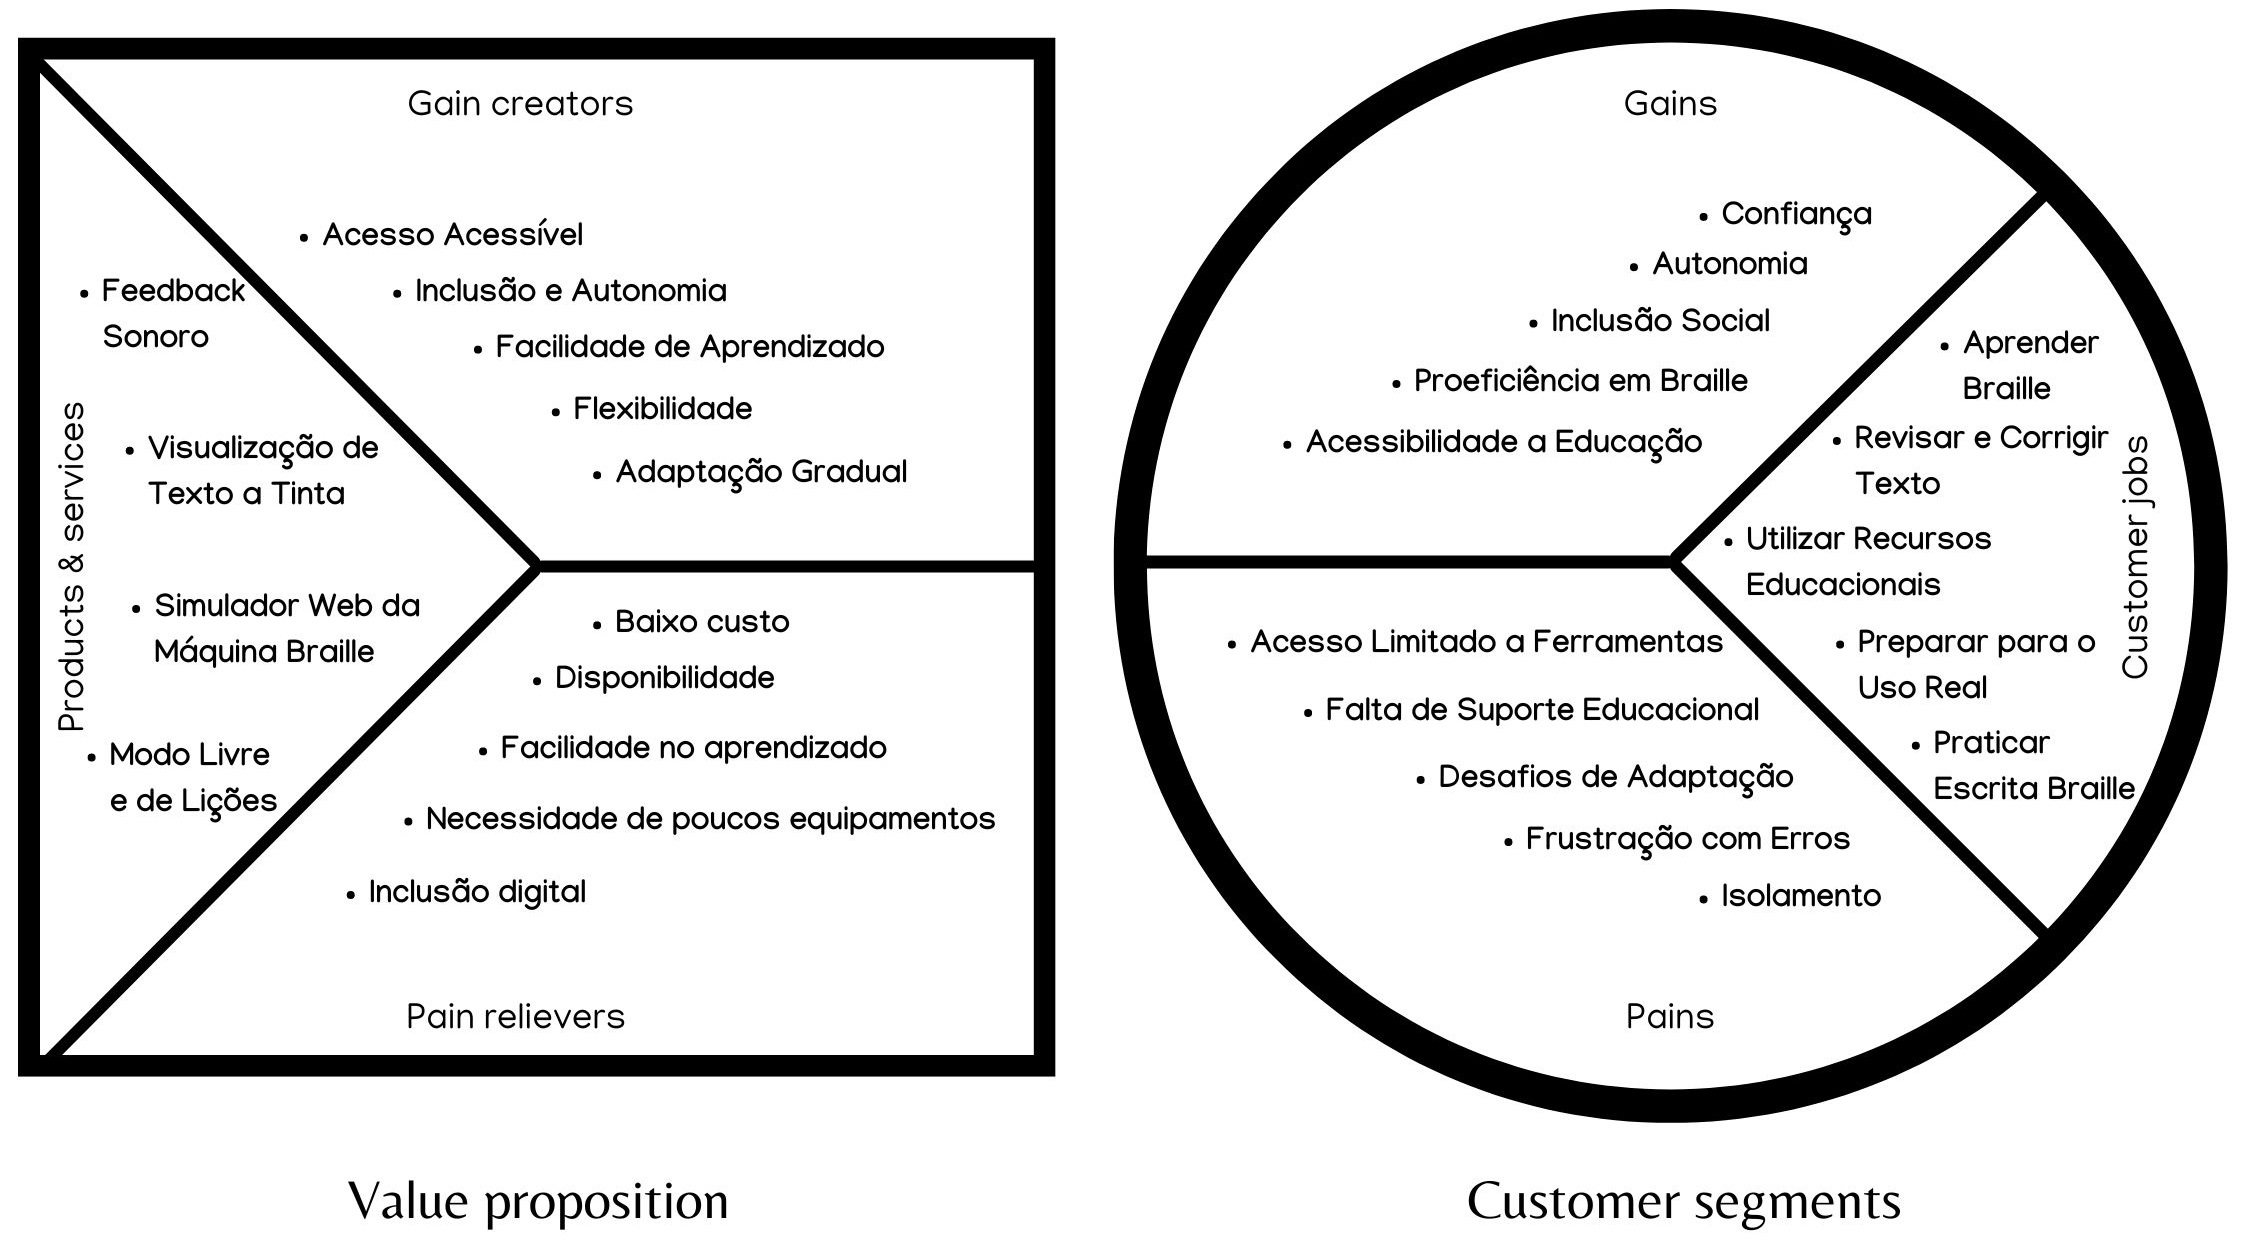
\includegraphics[scale=0.15]{ch03/assets/value-proposition.jpg}
    \decoRule
    \caption[Proposta de valor]{Proposta de valor}
    \label{fig:ch02-longitudinal-perspective}
\end{figure}

\subsubsection{Tarefas do Cliente}

Os clientes da aplicação têm como principal tarefa aprender a ler e escrever em Braille de maneira eficiente. Eles precisam praticar regularmente para ganhar fluência e confiança na escrita Braille. Outra tarefa importante é se preparar para o uso de uma Máquina Braille física, ganhando familiaridade com a disposição das teclas e os padrões de escrita. A revisão e correção do texto escrito são facilitadas pela navegação com as setas do teclado, melhorando a precisão e a qualidade da escrita. Além disso, os clientes utilizam os recursos educacionais fornecidos pela aplicação, aproveitando as lições e exercícios estruturados para aprimorar seu conhecimento e habilidade em Braille.

\subsubsection{Ganhos}

Com o uso da aplicação, os clientes aumentam significativamente sua proficiência em ler e escrever em Braille. Essa habilidade promove maior autonomia, permitindo que se comuniquem de forma independente utilizando Braille. A inclusão social é outro ganho importante, pois os usuários podem participar plenamente de atividades educacionais e profissionais que requerem o uso do Braille. 

A autoconfiança dos usuários também aumenta à medida que se tornam mais competentes na escrita Braille. Além disso, a aplicação oferece acesso a materiais educativos e oportunidades de aprendizado sem a necessidade de equipamentos caros, facilitando a educação contínua em Braille.

\subsubsection{Dores}

Antes da existência da aplicação, muitos enfrentavam acesso limitado a ferramentas de aprendizado de Braille devido ao alto custo das Máquinas Braille. A falta de suporte educacional adequado também é um problema significativo, dificultando o aprendizado de Braille. Cometer erros frequentes na escrita em Braille sem um sistema de correção acessível causa frustração, e o sentimento de isolamento é comum entre aqueles que não podiam participar plenamente de atividades que requerem o conhecimento do Braille.

\subsubsection{Produtos e Serviços}

A aplicação oferece uma interface interativa que permite aos usuários praticarem a escrita Braille usando o teclado do computador. Com dois modos de operação distintos, o Modo Livre permite a prática livre, onde os usuários podem escrever e visualizar o texto em células Braille sem restrições. O Modo de Lições oferece uma série de exercícios e lições estruturadas para facilitar o aprendizado do sistema Braille e o uso da Máquina Braille. 

Adicionalmente, a aplicação inclui uma funcionalidade que traduz o texto Braille para texto a tinta, tornando-o legível para aqueles que não estão familiarizados com Braille. Para aprimorar a experiência de aprendizado, a aplicação fornece feedback sonoro indicando qual caractere foi escrito, e permite a navegação pelo texto usando as setas do teclado, facilitando a revisão e correção do texto.

\subsubsection{Criadores de Ganho}

A aplicação é acessível ao aprendizado de Braille, pois elimina os custos associados à compra de uma Máquina Braille física. Ao oferecer uma ferramenta prática e gratuita, promove a inclusão e autonomia das pessoas com deficiência visual, permitindo que pratiquem de forma independente. A estrutura de lições e exercícios facilita o aprendizado, tornando-o mais eficiente e interativo. A flexibilidade de poder praticar a qualquer hora e em qualquer lugar, sem a necessidade de equipamento especializado, é uma grande vantagem. Além disso, a aplicação prepara gradualmente o usuário para a transição ao uso de uma Máquina Braille real, tornando o processo menos intimidante e mais confortável.

\subsubsection{Alívio das Dores}

A aplicação elimina a barreira do custo elevado das Máquinas Braille físicas, tornando o aprendizado de Braille mais acessível. Ao fornecer um recurso facilmente acessível e disponível online, resolve a falta de recursos adequados para o aprendizado de Braille. A interface amigável e o feedback contínuo simplificam o processo de aprendizagem, aliviando a dificuldade associada ao aprendizado de um novo sistema de escrita. 

Para ambientes educacionais, a aplicação remove a necessidade de múltiplas Máquinas Braille físicas, permitindo práticas em grupo de forma virtual e inclusiva. Finalmente, ao oferecer uma solução tecnológica moderna, a aplicação promove a inclusão digital, permitindo que qualquer pessoa com um computador e teclado possa aprender Braille.

\section{Valor para o cliente}

O Canvas Business Model é uma ferramenta estratégica desenvolvida por Alexander Osterwalder e Yves Pigneur, projetada para ajudar empresas a delinear, visualizar e inovar seus modelos de negócio. O Canvas Business Model se tornou amplamente utilizado tanto na academia quanto na prática empresarial. 

A ferramenta divide um modelo de negócio em nove blocos principais: segmentos de clientes, proposição de valor, canais, relacionamento com clientes, fontes de receita, recursos-chave, atividades-chave, parcerias-chave e estrutura de custos. Essa divisão incentiva os empreendedores a analisar cada elemento do negócio de forma detalhada e integrada, promovendo a reflexão constante, criatividade e inovação. 

Esta seção aborda o valor da aplicação para o cliente de forma mais profunda, utilizando a estrutura do Canvas Business Model. Essa análise  é crucial para entender como a aplicação atenderá às necessidades de seus usuários, promovendo a inclusão e autonomia de pessoas com deficiência visual.


\begin{figure}[h]
    \centering
    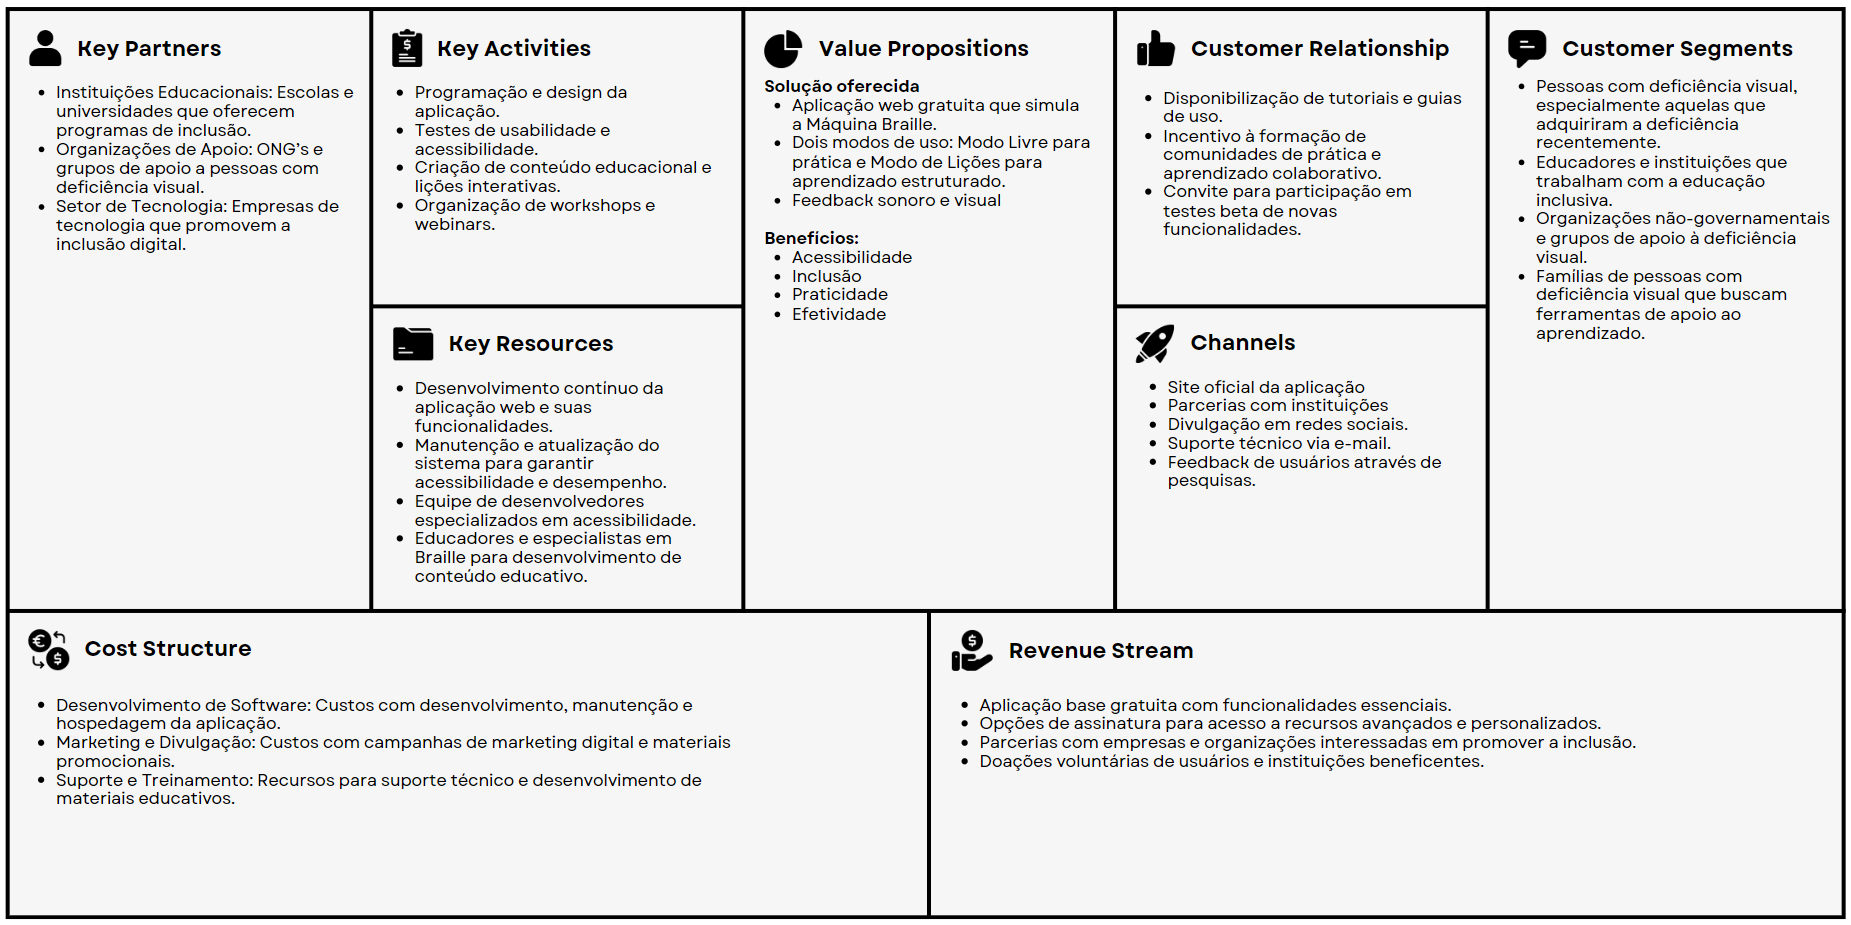
\includegraphics[scale=0.3]{ch03/assets/canva-business-model.png}
    \decoRule
    \caption[Canvas Business Model]{Canvas Business Model}
    \label{fig:ch02-canva-business-model}
\end{figure}

\section{Sumário}

Esta capítulo detalhou o valor da aplicação Web simuladora da Máquina de Escrever em Braille. A aplicação oferece uma solução prática, acessível e inclusiva, promovendo a autonomia de pessoas com deficiência visual e facilitando o aprendizado do Braille de maneira eficaz.



\chapter{Experimentação e Avaliação} 
\label{chap:Chapter04}

A avaliação da aplicação é essencial para garantir sua eficácia, acessibilidade e usabilidade. Este capítulo descreve o plano de experimentação e avaliação adotado para testar e validar a aplicação. Para isso, será utilizado o método GQM (Goals, Questions, Metrics), além de outros testes de acessibilidade.

\section{Metodologia de Avaliação}

\subsection{Hipótese de Investigação}

A avaliação do projeto terá como base a seguinte hipótese: O uso da do simulador da Máquina Braille melhora a aprendizagem do Braille e do uso da Máquina Braille.

\subsection{Goals, Questions, Metrics}

O método \textit{"Goal Question Metric"} (GQM) é uma abordagem que ajuda organizações a medir seus processos de forma eficaz \parencite{ARTICLE13}. Ele começa com a definição clara dos objetivos da organização e de seus projetos. Em seguida, esses objetivos são relacionados a perguntas específicas que orientam a coleta de dados relevantes. Finalmente, os dados coletados são analisados para interpretar se os objetivos foram alcançados.

\begin{figure}[h]
    \centering
    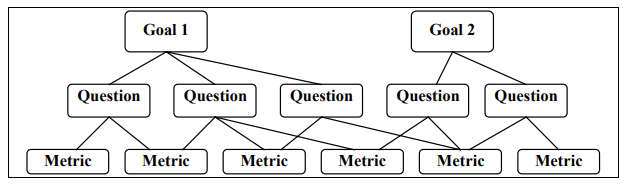
\includegraphics[scale=0.5]{ch04/assets/gqm.png}
    \decoRule
    \caption[Goal, Question, Metric]{Goal, Question, Metric \parencite{ARTICLE13}}
    \label{fig:ch02-gqm}
\end{figure}

A metodologia GQM será utilizada para definir objetivos claros, formular questões relevantes e identificar métricas adequadas para medir o desempenho da aplicação. Na tabela \ref{tab:GQM}, são apresentados os objetivos, as perguntas e as métricas que serão utilizadas na avaliação.

\begin{table}[h]
    \caption{Goals, Questions and Metrics}
    \label{tab:GQM}
    \centering
    \begin{tabular}{|p{0.2\linewidth}|p{0.35\linewidth}|p{0.35\linewidth}|} \hline 
         \textbf{Goal} & \textbf{Questions} & \textbf{Metrics} \\ \hline
        \textbf{(G1) Avaliar a Usabilidade da Aplicação} & 
        \begin{itemize}
            \item (Q1) Os usuários conseguem utilizar a aplicação de forma intuitiva?
            \item (Q2) A interface da aplicação é amigável e fácil de usar?
        \end{itemize} & 
        \begin{itemize}
            \item (M1) Número de erros cometidos pelos usuários ao tentar usar as funcionalidades básicas.
            \item (M2) Tempo médio para completar uma lição ou tarefa específica.
            \item (M3) Pontuação média em questionários de satisfação dos usuários.
            \item (M4) Comentários qualitativos sobre a experiência de uso.
        \end{itemize} \\ \hline
        
        \textbf{(G2) Avaliar a Eficácia no Aprendizado do Braille} & 
        \begin{itemize}
            \item (Q3) A aplicação ajuda os usuários a aprender e praticar Braille de maneira eficaz?
            \item (Q4) Os usuários conseguem transitar do uso da aplicação para o uso de uma máquina Braille real de forma eficiente?
        \end{itemize} & 
        \begin{itemize}
            \item (M5) Percentual de acertos em testes de conhecimento de Braille antes e depois do uso da aplicação.
            \item (M6) Tempo médio para os usuários completarem lições com sucesso ao longo do tempo.
            \item (M7) Feedback dos usuários sobre a transição para a máquina Braille real.
            \item (M8) Número de tentativas necessárias para os usuários realizarem corretamente tarefas em uma máquina Braille real após praticarem com a aplicação.
        \end{itemize} \\ \hline
        
        \textbf{(G3) Avaliar a Acessibilidade da Aplicação} & 
        \begin{itemize}
            \item (Q5) A aplicação é acessível para pessoas com deficiência visual?
            \item (Q6) Os recursos de acessibilidade, como feedback sonoro, são eficazes?
        \end{itemize} & 
        \begin{itemize}
            \item (M9) Conformidade com as Diretrizes de Acessibilidade para Conteúdo Web (WCAG) 2.1.
            \item (M10) Resultados de testes de acessibilidade automatizados e manuais.
            \item (M11) Feedback qualitativo dos usuários sobre os recursos de acessibilidade.
        \end{itemize} \\ \hline
    \end{tabular}
\end{table}

A figura \ref{fig:ch04-map-gqm} mostra a relação dos objetivos, questionamentos e métricas.

\begin{figure}[h]
    \centering
    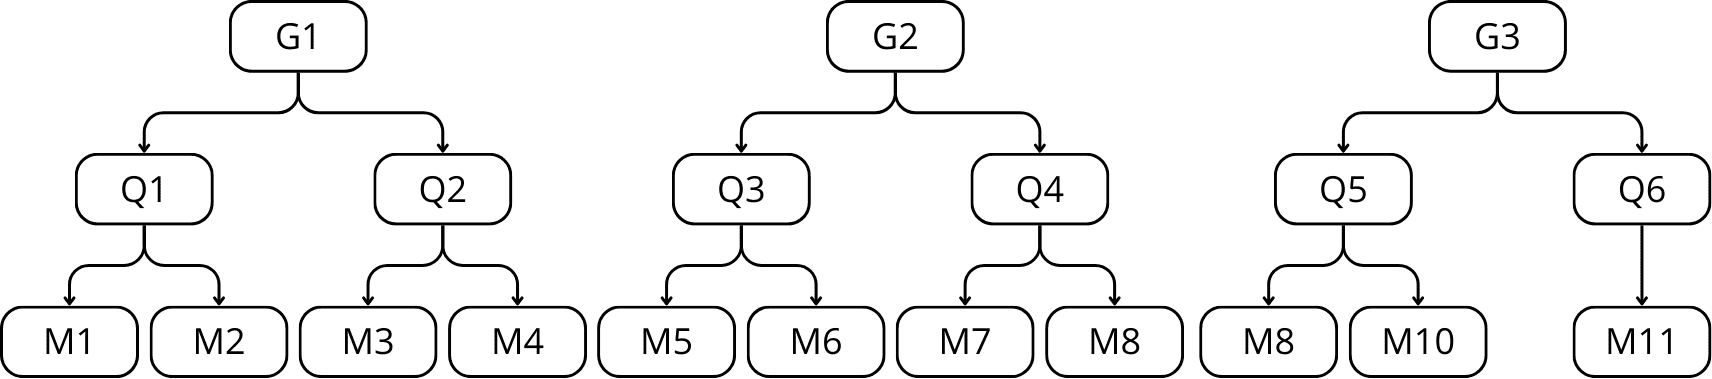
\includegraphics[scale=0.3]{ch04/assets/map-gqm.png}
    \decoRule
    \caption[Mapa do GQM]{Mapa do GQM}
    \label{fig:ch04-map-gqm}
\end{figure}

\section{Procedimentos de avaliação}

\subsection{Seleção de Participantes}

Os participantes dos testes serão selecionados visando obter uma amostra diversificada que represente diferentes perfis de usuários e ofereça insights abrangentes sobre a usabilidade, eficácia no aprendizado e acessibilidade da aplicação. Serão consideradas três categorias principais de participantes:

\begin{enumerate}
    \item \textbf{Usuários com Deficiência Visual:} Esta categoria abrangerá indivíduos que são cegos ou possuem baixa visão, tanto aqueles que adquiriram a deficiência recentemente quanto os que já possuem familiaridade com o Braille. A inclusão destes participantes permitirá avaliar como a aplicação atende às necessidades específicas de pessoas com deficiência visual, além de sua eficácia em promover o aprendizado e a prática do Braille de forma inclusiva.

    \item \textbf{Usuários sem Deficiência Visual:} Esta categoria englobará pessoas sem deficiência visual que desejam aprender Braille por motivos educacionais, profissionais ou de interesse pessoal. A participação destes usuários fornecerá insights sobre a experiência daqueles que estão sendo introduzidos ao Braille pela primeira vez, bem como sua percepção sobre a usabilidade e eficácia da aplicação.

    \item \textbf{Instrutores e Educadores:} Professores e instrutores especializados no ensino de Braille serão convidados a participar dos testes para oferecer uma perspectiva educacional sobre a aplicação. Esses profissionais possuem conhecimento especializado sobre as melhores práticas de ensino do Braille e podem oferecer insights sobre a eficácia pedagógica da aplicação, sua adequação para uso em ambientes educacionais e possíveis melhorias para otimizar a experiência de aprendizado dos alunos.
\end{enumerate}

Será assegurado que todos os participantes estejam confortáveis e seguros ao participarem dos testes, e qualquer preocupação com acessibilidade será atendida para garantir uma participação equitativa e significativa.

\subsection{Ambiente de Teste}

Os testes serão realizados em um ambiente que forneça condições ideais para a avaliação da aplicação. O ambiente de teste para cada usuário será em uma sala equipada com um computador de mesa com a aplicação, que conterá um teclado, um mouse, fones de ouvido ou caixas de som (dependendo da preferência do usuário).

O ambiente de teste será projetado para garantir a privacidade e o conforto dos participantes. Será reservado um tempo adequado para que os participantes possam familiarizar-se com a aplicação antes de iniciar os testes.

\subsection{Procedimentos de testes}

\subsubsection{Testes de Usabilidade}

Os testes de usabilidade serão conduzidos com o objetivo de avaliar a facilidade de uso e a intuitividade da aplicação. Os participantes serão solicitados a realizar uma série de tarefas específicas, como escrever palavras simples em Braille, utilizar a funcionalidade de quebra de linha e navegar pelo texto. 

Durante a realização dessas tarefas, serão registrados o número de erros cometidos pelos usuários e o tempo necessário para completar cada tarefa. Além disso, ao final dos testes, os participantes preencherão um questionário de satisfação, avaliando de 1 a 5 os seguintes aspectos da interface e usabilidade da aplicação: 

\begin{itemize}
    \item Clareza das instruções;
    \item Organização das funcionalidades
    \item Facilidade de aprendizado
\end{itemize}

\subsubsection{Testes de Eficácia no Aprendizado}

Os testes de eficácia no aprendizado têm como objetivo avaliar a capacidade da aplicação de facilitar o aprendizado do Braille e melhorar as habilidades dos usuários na escrita em Braille. Para isso, os participantes realizarão um teste de conhecimento antes e após o uso da aplicação, nos quais serão apresentadas questões relacionadas ao contexto do Braille e da Máquina Braille:

\begin{enumerate}
    \item Qual é a principal função do Sistema Braille?
    \item Quantos pontos compõem uma célula Braille?
    \item A Máquina Braille é formada por quais teclas?
    \item Quais pontos formam cada letra do seu nome no Sistema Braille?
    \item Qual sinal é utilizado para representar os números no sistema Braille?
    \item Quais são os sinais de pontuação mais comuns no Braille e como são representados?
    \item Como a máquina de escrever em Braille facilita a produção de textos em Braille?
\end{enumerate}

A diferença entre as pontuações obtidas nos dois testes indicará o progresso no aprendizado após a utilização da aplicação. Além disso, os participantes completarão uma série de lições e exercícios dentro da aplicação, com o progresso sendo monitorado ao longo do tempo para avaliar a eficácia do aprendizado.

\subsubsection{Testes de Acessibilidade}

Os testes de acessibilidade visam garantir que a aplicação seja acessível para pessoas com deficiência visual, permitindo que elas a utilizem de forma eficiente e autônoma. A acessibilidade será avaliada em conformidade com as Diretrizes de Acessibilidade para Conteúdo Web (WCAG) 2.1, utilizando tanto ferramentas automatizadas quanto inspeção manual. Serão verificados aspectos como o contraste de cores, a legibilidade do texto, a navegabilidade por meio de teclado e a compatibilidade com leitores de tela. 

Além disso, serão coletados feedbacks qualitativos dos usuários sobre a acessibilidade da aplicação, focalizando na eficácia dos recursos de feedback sonoro e na facilidade de navegação.



%----------------------------------------------------------------------------------------
%	BIBLIOGRAPHY
%----------------------------------------------------------------------------------------

\printbibliography[heading=bibintoc]

%----------------------------------------------------------------------------------------
%	THESIS CONTENT - APPENDICES
%----------------------------------------------------------------------------------------

\appendix % Cue to tell LaTeX that the following "chapters" are Appendices

% Include the appendices of the thesis as separate files from the Appendices folder
% Uncomment the lines as you write the Appendices

% \input{appendices/appendixA}
%\input{appendices/appendixB}
%\input{appendices/appendixC}

%----------------------------------------------------------------------------------------

\end{document}
